\documentclass[10pt]{article}
\usepackage[margin=2.2cm]{geometry}
\usepackage{amsmath,booktabs,graphicx,hyperref,array,float,caption}
\usepackage[numbers,sort&compress]{natbib}
% generated by scripts/make_tables.py - do not edit
\newcommand{\nDraws}{8\,000}
\newcommand{\nAccepted}{181}
\newcommand{\accPct}{2.3}
\newcommand{\postdzero}{1.9\;[1.1,\,7.8]}
\newcommand{\postbzero}{26.9\;[5.9,\,82.4]}
\newcommand{\postkd}{-20.5\;[-51.7,\,-9.2]}
\newcommand{\postkb}{-28.3\;[-167.9,\,36.6]}
\newcommand{\fracBzeroPos}{95}
\newcommand{\fracKbNeg}{75}
\newcommand{\nMarginalDraws}{300}
\newcommand{\marginalAllEnforced}{4.0}
\newcommand{\margAOne}{75}
\newcommand{\margATwo}{75}
\newcommand{\margAThree}{29}
\newcommand{\margAFive}{10}
\newcommand{\margAFour}{7}
\newcommand{\margASix}{13}
\newcommand{\failAone}{2127}
\newcommand{\failAthree}{3814}
\newcommand{\secAnchored}{448}
\newcommand{\nAccLoose}{62}
\newcommand{\nDrawsLoose}{3000}
\newcommand{\accPctLoose}{2.1}
\newcommand{\nAccStrict}{58}
\newcommand{\nDrawsStrict}{4000}
\newcommand{\accPctStrict}{1.5}
\newcommand{\nAccChen}{0}
\newcommand{\nDrawsChen}{4000}
\newcommand{\accPctChen}{0.0}
\newcommand{\nDesignWorlds}{181}
\newcommand{\tabDesigns}{\begin{tabular}{lccccc}\toprule design & mean yield & [10\%,90\% of worlds] & $P(\text{yield}\ge0.5)$ & mean $P(\text{switch})$ & median $\mu_{sw}$\\\midrule
circle & 0.00 & [0.00, 0.00] & 0.00 & 0.00 & 1.78 \\
square & 0.00 & [0.00, 0.00] & 0.00 & 0.01 & 1.25 \\
symmetric cross & 0.00 & [0.00, 0.01] & 0.00 & 0.02 & 1.21 \\
1:0.7, 0$^\circ$ & 0.00 & [0.00, 0.00] & 0.00 & 0.00 & 1.81 \\
1:0.7, 30$^\circ$ & 0.02 & [0.00, 0.00] & 0.02 & 0.07 & 1.51 \\
1:0.7, 60$^\circ$ & 0.30 & [0.00, 0.88] & 0.25 & 0.55 & 1.27 \\
1:0.7, 90$^\circ$ & 0.43 & [0.03, 0.93] & 0.42 & 0.58 & 1.69 \\
1:0.6, 0$^\circ$ & 0.00 & [0.00, 0.00] & 0.00 & 0.00 & 1.92 \\
1:0.6, 90$^\circ$ & 0.06 & [0.00, 0.14] & 0.05 & 0.10 & 1.98 \\
\midrule
mask A, 0$^\circ$ & 0.00 & [0.00, 0.00] & 0.00 & 0.00 & 1.90 \\
mask A, 30$^\circ$ & 0.03 & [0.00, 0.00] & 0.03 & 0.08 & 1.45 \\
mask A, 45$^\circ$ & 0.09 & [0.00, 0.27] & 0.08 & 0.17 & 1.28 \\
mask A, 60$^\circ$ & 0.32 & [0.00, 0.90] & 0.29 & 0.58 & 1.28 \\
mask A, 90$^\circ$ & 0.43 & [0.03, 0.94] & 0.43 & 0.58 & 1.69 \\
mask A, 120$^\circ$ & 0.32 & [0.00, 0.84] & 0.28 & 0.57 & 1.29 \\
mask A, 135$^\circ$ & 0.09 & [0.00, 0.23] & 0.08 & 0.18 & 1.24 \\
mask A, 150$^\circ$ & 0.03 & [0.00, 0.00] & 0.03 & 0.08 & 1.44 \\
mask B, 0$^\circ$ & 0.00 & [0.00, 0.00] & 0.00 & 0.00 & 1.75 \\
mask B, 30$^\circ$ & 0.01 & [0.00, 0.00] & 0.01 & 0.05 & 1.40 \\
mask B, 45$^\circ$ & 0.06 & [0.00, 0.14] & 0.05 & 0.14 & 1.31 \\
mask B, 60$^\circ$ & 0.25 & [0.00, 0.86] & 0.25 & 0.43 & 1.43 \\
mask B, 90$^\circ$ & 0.13 & [0.00, 0.76] & 0.12 & 0.19 & 1.98 \\
mask B, 120$^\circ$ & 0.24 & [0.00, 0.78] & 0.25 & 0.41 & 1.46 \\
mask B, 135$^\circ$ & 0.06 & [0.00, 0.17] & 0.05 & 0.14 & 1.29 \\
mask B, 150$^\circ$ & 0.01 & [0.00, 0.00] & 0.01 & 0.05 & 1.31 \\
\bottomrule\end{tabular}}
\newcommand{\noWorkingSeven}{9}
\newcommand{\tabTopSeven}{\begin{tabular}{lc}\toprule design of APL 126 & share of worlds in which it is the best of the seven\\\midrule
square & 0\% \\
1:0.7, 0$^\circ$ & 0\% \\
1:0.7, 30$^\circ$ & 2\% \\
1:0.7, 60$^\circ$ & 31\% \\
1:0.7, 90$^\circ$ & 54\% \\
1:0.6, 0$^\circ$ & 0\% \\
1:0.6, 90$^\circ$ & 4\% \\
\bottomrule\end{tabular}}
\newcommand{\bestThetaSeven}{70}
\newcommand{\plateauLo}{70}
\newcommand{\plateauHi}{110}
\newcommand{\meanYieldSevenMax}{0.47}
\newcommand{\reachRatioFive}{9}
\newcommand{\reachRatioSix}{34}
\newcommand{\reachRatioSeven}{74}
\newcommand{\reachRatioEight}{24}
\newcommand{\reachRatioNine}{1}
\newcommand{\pswZero}{0.00}
\newcommand{\yldZero}{0.00}
\newcommand{\geZero}{0.00}
\newcommand{\pswThirty}{0.07}
\newcommand{\yldThirty}{0.02}
\newcommand{\geThirty}{0.02}
\newcommand{\pswSixty}{0.55}
\newcommand{\yldSixty}{0.30}
\newcommand{\geSixty}{0.25}
\newcommand{\pswNinety}{0.58}
\newcommand{\yldNinety}{0.43}
\newcommand{\geNinety}{0.42}
\newcommand{\pswSym}{0.02}
\newcommand{\yldSym}{0.00}
\newcommand{\geSym}{0.00}
\newcommand{\pswCircle}{0.00}
\newcommand{\yldCircle}{0.00}
\newcommand{\geCircle}{0.00}
\newcommand{\pswSquare}{0.01}
\newcommand{\yldSquare}{0.00}
\newcommand{\geSquare}{0.00}
\newcommand{\tabWindow}{\begin{tabular}{lccccccccc}\toprule window ($\mu_{sw}$) & 40$^\circ$ & 50$^\circ$ & 60$^\circ$ & 70$^\circ$ & 80$^\circ$ & 90$^\circ$ & best & $P(60^\circ>90^\circ)$ & $P(90^\circ>60^\circ)$\\\midrule
default 1.25-1.95 & 0.05 & 0.12 & 0.27 & 0.43 & 0.40 & 0.39 & 70$^\circ$ & 0.31 & 0.63 \\
low bias 1.15-1.60 & 0.05 & 0.11 & 0.27 & 0.39 & 0.27 & 0.23 & 70$^\circ$ & 0.53 & 0.43 \\
wide 1.15-2.05 & 0.07 & 0.16 & 0.36 & 0.54 & 0.48 & 0.46 & 70$^\circ$ & 0.35 & 0.60 \\
mid 1.50-1.70 & 0.01 & 0.04 & 0.06 & 0.12 & 0.13 & 0.12 & 80$^\circ$ & 0.23 & 0.62 \\
\bottomrule\end{tabular}}
\newcommand{\nWindowWorlds}{91}
\newcommand{\lowBiasSixtyBeatsNinety}{53}
\newcommand{\lowBiasNinetyBeatsSixty}{43}
\newcommand{\defSixtyBeatsNinety}{31}
\newcommand{\defNinetyBeatsSixty}{63}
\newcommand{\rotRobustBest}{80}
\newcommand{\rotRobustBestShare}{0.91}
\newcommand{\nRotWorking}{6}
\newcommand{\shareSixtyLo}{40}
\newcommand{\shareSixtyHi}{68}
\newcommand{\shareOneTwentyLo}{38}
\newcommand{\shareOneTwentyHi}{65}
\newcommand{\rotWorstSevenZero}{0.79}
\newcommand{\rotWorstEightZero}{0.91}
\newcommand{\rotWorstNineZero}{0.87}
\newcommand{\tabRotSets}{\begin{tabular}{lcccccccccccccc}\toprule world set & worlds & 40$^\circ$ & 50$^\circ$ & 60$^\circ$ & 70$^\circ$ & 80$^\circ$ & 90$^\circ$ & 100$^\circ$ & 110$^\circ$ & 120$^\circ$ & 130$^\circ$ & 140$^\circ$ & best & within 90\,\% of best\\\midrule
primary (every third world) & 40 & 0.03 & 0.09 & 0.33 & 0.53 & 0.49 & 0.47 & 0.49 & 0.54 & 0.32 & 0.09 & 0.02 & 110$^\circ$ & 70--110$^\circ$ \\
loose thresholds & 40 & 0.02 & 0.04 & 0.33 & 0.48 & 0.47 & 0.43 & 0.47 & 0.49 & 0.31 & 0.04 & 0.02 & 110$^\circ$ & 70--110$^\circ$ \\
strict thresholds & 40 & 0.04 & 0.11 & 0.38 & 0.58 & 0.67 & 0.63 & 0.67 & 0.59 & 0.38 & 0.11 & 0.04 & 80$^\circ$ & 80--100$^\circ$ \\
wider prior & 40 & 0.07 & 0.14 & 0.29 & 0.44 & 0.49 & 0.49 & 0.49 & 0.44 & 0.29 & 0.14 & 0.07 & 80$^\circ$ & 80--110$^\circ$ \\
re-inferred, isotropic oxidation ($\eta=1.0$) & 40 & 0.06 & 0.11 & 0.24 & 0.44 & 0.46 & 0.49 & 0.47 & 0.45 & 0.23 & 0.11 & 0.06 & 90$^\circ$ & 70--110$^\circ$ \\
re-inferred, $\eta=1.3$ & 40 & 0.05 & 0.10 & 0.21 & 0.42 & 0.53 & 0.53 & 0.53 & 0.42 & 0.20 & 0.09 & 0.05 & 80$^\circ$ & 80--100$^\circ$ \\
re-inferred, thermal drift $\chi_{th}=-0.2$ & 40 & 0.02 & 0.02 & 0.02 & 0.01 & 0.03 & 0.05 & 0.03 & 0.02 & 0.02 & 0.02 & 0.02 & 90$^\circ$ & 90--90$^\circ$ \\
re-inferred, thermal drift $\chi_{th}=+0.2$ & 40 & 0.01 & 0.01 & 0.03 & 0.03 & 0.01 & 0.01 & 0.01 & 0.03 & 0.03 & 0.01 & 0.01 & 70$^\circ$ & 70--70$^\circ$ \\
worst case over the 6 working sets (share of best) & & 0.04 & 0.09 & 0.40 & 0.79 & 0.91 & 0.87 & 0.90 & 0.78 & 0.38 & 0.08 & 0.03 & 80$^\circ$ & \\
\bottomrule\end{tabular}}
\newcommand{\rotSetsBestLo}{70}
\newcommand{\rotSetsBestHi}{110}
\newcommand{\nRotSets}{8}
\newcommand{\pHighestSeventy}{13}
\newcommand{\worstMeanSeventy}{0.75}
\newcommand{\worstLoSeventy}{0.61}
\newcommand{\worstHiSeventy}{0.88}
\newcommand{\pHighestEighty}{80}
\newcommand{\worstMeanEighty}{0.86}
\newcommand{\worstLoEighty}{0.70}
\newcommand{\worstHiEighty}{0.97}
\newcommand{\pHighestNinety}{7}
\newcommand{\worstMeanNinety}{0.81}
\newcommand{\worstLoNinety}{0.64}
\newcommand{\worstHiNinety}{0.93}
\newcommand{\pEightyAboveNinety}{93}
\newcommand{\pEightyAboveSeventy}{87}
\newcommand{\nBootRot}{2000}
\newcommand{\wideBest}{80}
\newcommand{\wideMax}{0.49}
\newcommand{\nAccPrim}{181}
\newcommand{\dzeroMedPrim}{1.95}
\newcommand{\dzeroQfivePrim}{1.06}
\newcommand{\dzeroQninetyfivePrim}{7.83}
\newcommand{\dzeroNearEdgePrim}{53}
\newcommand{\nAccWide}{101}
\newcommand{\dzeroMedWide}{0.81}
\newcommand{\dzeroQfiveWide}{0.22}
\newcommand{\dzeroQninetyfiveWide}{5.76}
\newcommand{\dzeroNearEdgeWide}{24}
\newcommand{\accPctWide}{2.5}
\newcommand{\dzeroBelowOneWide}{60}
\newcommand{\dzeroBelowHalfWide}{31}
\newcommand{\nDrawsWide}{4000}
\newcommand{\nAccOxTen}{56}
\newcommand{\nDrawsOxTen}{4000}
\newcommand{\fracBzeroPosOxTen}{89}
\newcommand{\nAccOxThirteen}{70}
\newcommand{\nDrawsOxThirteen}{4000}
\newcommand{\fracBzeroPosOxThirteen}{97}
\newcommand{\nAccChiMinus}{116}
\newcommand{\nDrawsChiMinus}{4000}
\newcommand{\fracBzeroPosChiMinus}{97}
\newcommand{\nAccChiPlus}{126}
\newcommand{\nDrawsChiPlus}{4000}
\newcommand{\fracBzeroPosChiPlus}{4}
\newcommand{\nRunsPone}{20}
\newcommand{\nRunsPthree}{8}
\newcommand{\tabBench}{\begin{tabular}{lccc}\toprule & P1 (default window) & P2 (narrow window) & P3 (one design, unseen worlds)\\\midrule
random search & 0.81 [0.74, 0.88] & 0.33 [0.29, 0.37] & 0.39 [0.36, 0.42] \\
Sobol & 0.87 [0.80, 0.92] & 0.35 [0.30, 0.39] & 0.42 [0.38, 0.46] \\
differential evolution & 0.89 [0.84, 0.94] & 0.38 [0.34, 0.42] & 0.37 [0.32, 0.41] \\
GP-EI & 0.96 [0.92, 0.98] & 0.43 [0.38, 0.47] & 0.41 [0.36, 0.45] \\
GP-UCB & 0.86 [0.74, 0.96] & 0.43 [0.38, 0.48] & 0.40 [0.38, 0.43] \\
\bottomrule\end{tabular}}
\newcommand{\tabTests}{\begin{tabular}{llccc}\toprule problem & paired difference & mean diff. & Wilcoxon $p$ & pairs\\\midrule
P1 & GP-EI - random & +0.145 & 0.001 & 20 \\
P1 & GP-EI - Sobol & +0.090 & 0.001 & 20 \\
P1 & GP-EI - DE & +0.063 & 0.008 & 20 \\
P1 & GP-UCB - random & +0.046 & 0.083 & 20 \\
P1 & GP-UCB - Sobol & -0.009 & 0.171 & 20 \\
P1 & GP-UCB - DE & -0.036 & 0.475 & 20 \\
P2 & GP-EI - random & +0.100 & 0.001 & 40 \\
P2 & GP-EI - Sobol & +0.084 & 0.002 & 40 \\
P2 & GP-EI - DE & +0.047 & 0.075 & 40 \\
P2 & GP-UCB - random & +0.100 & 0.001 & 40 \\
P2 & GP-UCB - Sobol & +0.084 & 0.008 & 40 \\
P2 & GP-UCB - DE & +0.047 & 0.139 & 40 \\
P3 & GP-EI - random & +0.018 & 0.641 & 8 \\
P3 & GP-EI - Sobol & -0.014 & 0.844 & 8 \\
P3 & GP-EI - DE & +0.041 & 0.148 & 8 \\
P3 & GP-UCB - random & +0.012 & 0.641 & 8 \\
P3 & GP-UCB - Sobol & -0.020 & 0.547 & 8 \\
P3 & GP-UCB - DE & +0.035 & 0.250 & 8 \\
\bottomrule\end{tabular}}
\newcommand{\benchOneRandom}{0.81}
\newcommand{\benchOneSobol}{0.87}
\newcommand{\benchOneDe}{0.89}
\newcommand{\benchOneBoEi}{0.96}
\newcommand{\benchOneBoUcb}{0.86}
\newcommand{\benchTwoRandom}{0.33}
\newcommand{\benchTwoSobol}{0.35}
\newcommand{\benchTwoDe}{0.38}
\newcommand{\benchTwoBoEi}{0.43}
\newcommand{\benchTwoBoUcb}{0.43}
\newcommand{\benchThreeRandom}{0.39}
\newcommand{\benchThreeSobol}{0.42}
\newcommand{\benchThreeDe}{0.37}
\newcommand{\benchThreeBoEi}{0.41}
\newcommand{\benchThreeBoUcb}{0.40}
\newcommand{\diffOneBoEiRandom}{+0.14}
\newcommand{\pvalOneBoEiRandom}{0.001}
\newcommand{\diffOneBoEiSobol}{+0.09}
\newcommand{\pvalOneBoEiSobol}{0.001}
\newcommand{\diffOneBoEiDe}{+0.06}
\newcommand{\pvalOneBoEiDe}{0.008}
\newcommand{\diffOneBoUcbRandom}{+0.05}
\newcommand{\pvalOneBoUcbRandom}{0.083}
\newcommand{\diffOneBoUcbSobol}{-0.01}
\newcommand{\pvalOneBoUcbSobol}{0.171}
\newcommand{\diffOneBoUcbDe}{-0.04}
\newcommand{\pvalOneBoUcbDe}{0.475}
\newcommand{\diffTwoBoEiRandom}{+0.10}
\newcommand{\pvalTwoBoEiRandom}{0.001}
\newcommand{\diffTwoBoEiSobol}{+0.08}
\newcommand{\pvalTwoBoEiSobol}{0.002}
\newcommand{\diffTwoBoEiDe}{+0.05}
\newcommand{\pvalTwoBoEiDe}{0.075}
\newcommand{\diffTwoBoUcbRandom}{+0.10}
\newcommand{\pvalTwoBoUcbRandom}{0.001}
\newcommand{\diffTwoBoUcbSobol}{+0.08}
\newcommand{\pvalTwoBoUcbSobol}{0.008}
\newcommand{\diffTwoBoUcbDe}{+0.05}
\newcommand{\pvalTwoBoUcbDe}{0.139}
\newcommand{\diffThreeBoEiRandom}{+0.02}
\newcommand{\pvalThreeBoEiRandom}{0.641}
\newcommand{\diffThreeBoEiSobol}{-0.01}
\newcommand{\pvalThreeBoEiSobol}{0.844}
\newcommand{\diffThreeBoEiDe}{+0.04}
\newcommand{\pvalThreeBoEiDe}{0.148}
\newcommand{\diffThreeBoUcbRandom}{+0.01}
\newcommand{\pvalThreeBoUcbRandom}{0.641}
\newcommand{\diffThreeBoUcbSobol}{-0.02}
\newcommand{\pvalThreeBoUcbSobol}{0.547}
\newcommand{\diffThreeBoUcbDe}{+0.03}
\newcommand{\pvalThreeBoUcbDe}{0.250}
\newcommand{\friedOne}{0.00}
\newcommand{\nWorldsOne}{5}
\newcommand{\worldsBoAheadDeOne}{4}
\newcommand{\worldsDeAheadBoOne}{1}
\newcommand{\worldsTieBoDeOne}{0}
\newcommand{\friedTwo}{0.00}
\newcommand{\nWorldsTwo}{5}
\newcommand{\worldsBoAheadDeTwo}{3}
\newcommand{\worldsDeAheadBoTwo}{1}
\newcommand{\worldsTieBoDeTwo}{1}
\newcommand{\friedThree}{0.18}
\newcommand{\nWorldsThree}{1}
\newcommand{\worldsBoAheadDeThree}{1}
\newcommand{\worldsDeAheadBoThree}{0}
\newcommand{\worldsTieBoDeThree}{0}
\newcommand{\benchOneMin}{0.81}
\newcommand{\benchOneMax}{0.96}
\newcommand{\nRunsOne}{20}
\newcommand{\benchTwoMin}{0.33}
\newcommand{\benchTwoMax}{0.43}
\newcommand{\nRunsTwo}{40}
\newcommand{\benchThreeMin}{0.37}
\newcommand{\benchThreeMax}{0.42}
\newcommand{\nRunsThree}{8}
\newcommand{\lowRunsOneRandom}{1}
\newcommand{\lowRunsOneSobol}{1}
\newcommand{\lowRunsOneDe}{0}
\newcommand{\lowRunsOneBoEi}{0}
\newcommand{\lowRunsOneBoUcb}{3}
\newcommand{\nRunsOnePerMethod}{20}
\newcommand{\ucbLowBestMin}{0.20}
\newcommand{\ucbLowBestMax}{0.49}
\newcommand{\waferOneBoEiDe}{+0.06\;[-0.03,\,+0.15]}
\newcommand{\waferAheadOneBoEiDe}{4}
\newcommand{\waferOneBoEiRandom}{+0.14\;[+0.06,\,+0.23]}
\newcommand{\waferAheadOneBoEiRandom}{5}
\newcommand{\waferOneBoEiSobol}{+0.09\;[-0.00,\,+0.18]}
\newcommand{\waferAheadOneBoEiSobol}{5}
\newcommand{\waferOneBoUcbDe}{-0.04\;[-0.27,\,+0.20]}
\newcommand{\waferAheadOneBoUcbDe}{3}
\newcommand{\waferOneBoUcbRandom}{+0.05\;[-0.09,\,+0.18]}
\newcommand{\waferAheadOneBoUcbRandom}{3}
\newcommand{\waferOneBoUcbSobol}{-0.01\;[-0.11,\,+0.09]}
\newcommand{\waferAheadOneBoUcbSobol}{3}
\newcommand{\waferTwoBoEiDe}{+0.05\;[-0.06,\,+0.15]}
\newcommand{\waferAheadTwoBoEiDe}{4}
\newcommand{\waferTwoBoEiRandom}{+0.10\;[+0.02,\,+0.18]}
\newcommand{\waferAheadTwoBoEiRandom}{4}
\newcommand{\waferTwoBoEiSobol}{+0.08\;[-0.01,\,+0.18]}
\newcommand{\waferAheadTwoBoEiSobol}{5}
\newcommand{\waferTwoBoUcbDe}{+0.05\;[-0.04,\,+0.13]}
\newcommand{\waferAheadTwoBoUcbDe}{4}
\newcommand{\waferTwoBoUcbRandom}{+0.10\;[+0.03,\,+0.17]}
\newcommand{\waferAheadTwoBoUcbRandom}{5}
\newcommand{\waferTwoBoUcbSobol}{+0.08\;[+0.00,\,+0.16]}
\newcommand{\waferAheadTwoBoUcbSobol}{5}
\newcommand{\tabWafer}{\begin{tabular}{llccc}\toprule problem & comparison & mean over wafers & 95\,\% $t$-interval (4 d.f.) & wafers ahead\\\midrule
P1 & GP-EI $-$ differential evolution & +0.063 & [-0.028, +0.154] & 4 of 5 \\
P1 & GP-EI $-$ random search & +0.145 & [+0.063, +0.226] & 5 of 5 \\
P1 & GP-EI $-$ Sobol & +0.090 & [-0.001, +0.181] & 5 of 5 \\
P1 & GP-UCB $-$ differential evolution & -0.036 & [-0.269, +0.197] & 3 of 5 \\
P1 & GP-UCB $-$ random search & +0.046 & [-0.088, +0.180] & 3 of 5 \\
P1 & GP-UCB $-$ Sobol & -0.009 & [-0.112, +0.094] & 3 of 5 \\
P2 & GP-EI $-$ differential evolution & +0.047 & [-0.060, +0.154] & 4 of 5 \\
P2 & GP-EI $-$ random search & +0.100 & [+0.024, +0.176] & 4 of 5 \\
P2 & GP-EI $-$ Sobol & +0.084 & [-0.013, +0.181] & 5 of 5 \\
P2 & GP-UCB $-$ differential evolution & +0.047 & [-0.040, +0.133] & 4 of 5 \\
P2 & GP-UCB $-$ random search & +0.100 & [+0.035, +0.166] & 5 of 5 \\
P2 & GP-UCB $-$ Sobol & +0.084 & [+0.004, +0.164] & 5 of 5 \\
\bottomrule\end{tabular}}
\newcommand{\pThreeSelLo}{0.58}
\newcommand{\pThreeSelHi}{0.63}
\newcommand{\pThreeUnseenLo}{0.37}
\newcommand{\pThreeUnseenHi}{0.42}
\newcommand{\pThreeGapLo}{0.16}
\newcommand{\pThreeGapHi}{0.24}
\newcommand{\fracGoodRange}{0.02 -- 0.11}
\newcommand{\nTrainWorlds}{32}
\newcommand{\nTestWorlds}{32}
\newcommand{\nPool}{177}
\newcommand{\singleBestYield}{0.69}
\newcommand{\tabBatch}{\begin{tabular}{lcc}\toprule set of designs & $E[\text{best yield}]$ & $P(\text{some design}\ge0.5)$\\\midrule
greedy portfolio, 16 designs & 0.86 & 0.94 \\
first 8 designs of the portfolio & 0.85 & 0.94 \\
the seven designs of APL 126 & 0.57 & 0.59 \\
author's mask (16 designs) & 0.68 & 0.72 \\
rotation-only family (8, ratio 0.7) & 0.71 & 0.78 \\
16 random designs from the pool & 0.69 $\pm$ 0.12 & -- \\
best single design (mean yield) & 0.69 (mean) & 0.75 \\
\bottomrule\end{tabular}}
\newcommand{\noWorkingTest}{2}
\newcommand{\tabMaskPlus}{\begin{tabular}{lcc}\toprule & $E[\text{best yield}]$ & $P(\text{some design}\ge0.5)$\\\midrule
author's mask (16) & 0.68 & 0.72 \\
+ 1 added design & 0.84 & 0.88 \\
+ 2 added designs & 0.85 & 0.91 \\
+ 3 added designs & 0.85 & 0.91 \\
+ 4 added designs & 0.86 & 0.91 \\
+ 5 added designs & 0.86 & 0.91 \\
+ 6 added designs & 0.86 & 0.91 \\
+ 7 added designs & 0.87 & 0.94 \\
+ 8 added designs & 0.87 & 0.94 \\
\bottomrule\end{tabular}}
\newcommand{\tabAdd}{\begin{tabular}{cccccc}\toprule \# & $L$ ($\mu$m) & arm ratio & $w$ ($\mu$m) & $\rho$ & rotation ($^\circ$)\\\midrule
1 & 19.6 & 0.50 & 3.5 & 1.00 & 85 \\
2 & 17.4 & 0.72 & 6.2 & 0.82 & 70 \\
3 & 17.7 & 0.50 & 3.5 & 0.00 & 90 \\
4 & 18.6 & 0.78 & 6.3 & 0.52 & 80 \\
5 & 13.0 & 0.84 & 8.0 & 0.21 & 88 \\
6 & 17.5 & 0.64 & 4.4 & 0.94 & 36 \\
7 & 19.3 & 0.67 & 3.8 & 0.16 & 83 \\
8 & 17.5 & 0.70 & 6.0 & 0.50 & 112 \\
\bottomrule\end{tabular}}
\newcommand{\tabBatchList}{\begin{tabular}{clcccccccc}\toprule id & origin & $L$ & ratio & $w$ & $\rho$ & $\theta$ & $E$(yield) & $P(\ge0.5)$\\\midrule
0 & bo1 & 19.7 & 0.50 & 3.5 & 1.00 & 85 & 0.69 & 0.75 \\
1 & bo0 & 13.0 & 0.84 & 8.0 & 0.21 & 88 & 0.41 & 0.44 \\
2 & sobol & 18.6 & 0.78 & 6.3 & 0.52 & 80 & 0.26 & 0.22 \\
3 & sobol & 17.4 & 0.72 & 6.2 & 0.82 & 70 & 0.59 & 0.59 \\
4 & bo1 & 17.7 & 0.50 & 3.5 & 0.00 & 90 & 0.60 & 0.59 \\
5 & sobol & 17.4 & 0.50 & 4.3 & 0.10 & 100 & 0.21 & 0.19 \\
6 & sobol & 17.5 & 0.65 & 4.4 & 0.94 & 36 & 0.01 & 0.00 \\
7 & sobol & 19.3 & 0.67 & 3.8 & 0.16 & 83 & 0.41 & 0.47 \\
8 & rotfam & 17.5 & 0.70 & 6.0 & 0.50 & 112 & 0.51 & 0.56 \\
9 & bo1 & 19.6 & 0.50 & 3.5 & 1.00 & 85 & 0.70 & 0.75 \\
10 & sobol & 15.6 & 0.68 & 5.2 & 0.31 & 41 & 0.06 & 0.06 \\
11 & bo0 & 13.0 & 0.84 & 8.0 & 0.00 & 90 & 0.39 & 0.44 \\
12 & bo1 & 18.5 & 0.50 & 3.5 & 0.00 & 90 & 0.59 & 0.62 \\
13 & sobol & 14.4 & 0.75 & 5.8 & 0.53 & 112 & 0.48 & 0.53 \\
14 & mask:B45 & 15.0 & 0.70 & 6.0 & 0.75 & 45 & 0.03 & 0.03 \\
15 & bo1 & 19.4 & 0.50 & 3.5 & 1.00 & 86 & 0.69 & 0.78 \\
\bottomrule\end{tabular}}
\newcommand{\freshAnchorLo}{83}
\newcommand{\freshAnchorHi}{92}
\newcommand{\nFreshAnchorPops}{3}
\newcommand{\nOtherWorlds}{117}
\newcommand{\nNontrainWorlds}{149}
\newcommand{\othPortTest}{0.86}
\newcommand{\othPortOther}{0.74}
\newcommand{\othPortNon}{0.77}
\newcommand{\othPortEightTest}{0.85}
\newcommand{\othPortEightOther}{0.74}
\newcommand{\othPortEightNon}{0.76}
\newcommand{\othMaskTest}{0.68}
\newcommand{\othMaskOther}{0.61}
\newcommand{\othMaskNon}{0.63}
\newcommand{\othSevenTest}{0.57}
\newcommand{\othSevenOther}{0.56}
\newcommand{\othSevenNon}{0.56}
\newcommand{\othRotTest}{0.71}
\newcommand{\othRotOther}{0.60}
\newcommand{\othRotNon}{0.62}
\newcommand{\othMaskIntTest}{0.83}
\newcommand{\othMaskIntOther}{0.72}
\newcommand{\othMaskIntNon}{0.74}
\newcommand{\othMaskPoolTest}{0.85}
\newcommand{\othMaskPoolOther}{0.72}
\newcommand{\othMaskPoolNon}{0.75}
\newcommand{\othDiffPortMaskNon}{+0.14\;[+0.11,\,+0.17]}
\newcommand{\othDiffPortMaskOther}{+0.13\;[+0.09,\,+0.16]}
\newcommand{\othDiffPortSevenNon}{+0.20\;[+0.16,\,+0.24]}
\newcommand{\tabOther}{\begin{tabular}{lccc}\toprule set of designs & 32 test worlds (headline) & 117 other accepted worlds & all 149\\\midrule
greedy portfolio (16) & 0.86 & 0.74 & 0.77 \\
author's mask (16) & 0.68 & 0.61 & 0.63 \\
seven designs of APL 126 & 0.57 & 0.56 & 0.56 \\
rotation-only family (8) & 0.71 & 0.60 & 0.62 \\
author's mask + 3 interior additions & 0.83 & 0.72 & 0.74 \\
\bottomrule\end{tabular}}
\newcommand{\intMaskOnly}{0.68}
\newcommand{\intPlusOne}{0.78}
\newcommand{\intPlusTwo}{0.80}
\newcommand{\intPlusThree}{0.83}
\newcommand{\intPlusFour}{0.83}
\newcommand{\tabAddInterior}{\begin{tabular}{cccccccc}\toprule \# & $L$ ($\mu$m) & arm ratio & $w$ ($\mu$m) & $\rho$ & rotation ($^\circ$) & $E$(yield) alone & $E[\text{best}]$ of mask + \#\\\midrule
1 & 17.4 & 0.72 & 6.2 & 0.82 & 70 & 0.59 & 0.78 \\
2 & 18.6 & 0.78 & 6.3 & 0.52 & 80 & 0.26 & 0.80 \\
3 & 18.4 & 0.65 & 5.1 & 0.80 & 91 & 0.57 & 0.83 \\
4 & 17.5 & 0.70 & 6.0 & 0.50 & 112 & 0.51 & 0.83 \\
\bottomrule\end{tabular}}
\newcommand{\nWall}{8}
\newcommand{\nQ}{16}
\newcommand{\nPoolInterior}{81}
\newcommand{\nPoolAll}{177}
\newcommand{\freshDev}{48}
\newcommand{\freshPort}{0.86}
\newcommand{\freshPPort}{0.94}
\newcommand{\freshInt}{0.81}
\newcommand{\freshPInt}{0.91}
\newcommand{\freshMask}{0.67}
\newcommand{\freshPMask}{0.69}
\newcommand{\freshSeven}{0.58}
\newcommand{\freshPSeven}{0.59}
\newcommand{\interiorSame}{0.83}
\newcommand{\interiorSameP}{0.94}
\newcommand{\wallAreaLo}{34}
\newcommand{\wallAreaHi}{85}
\newcommand{\refAreaLo}{79}
\newcommand{\refAreaHi}{88}
\newcommand{\circleArea}{130}
\newcommand{\tabWalls}{\begin{tabular}{cccccccc}\toprule \# & $L$ & ratio & $w$ & $\rho$ & $\theta$ & aperture area ($\mu$m$^2$) & on a wall of the search box\\\midrule
0 & 19.7 & 0.50 & 3.5 & 1.00 & 85 & 37 & yes \\
1 & 13.0 & 0.84 & 8.0 & 0.21 & 88 & 84 & yes \\
2 & 18.6 & 0.78 & 6.3 & 0.52 & 80 & 108 &  \\
3 & 17.4 & 0.72 & 6.2 & 0.82 & 70 & 88 &  \\
4 & 17.7 & 0.50 & 3.5 & 0.00 & 90 & 34 & yes \\
5 & 17.4 & 0.50 & 4.3 & 0.10 & 100 & 48 & yes \\
6 & 17.5 & 0.65 & 4.4 & 0.94 & 36 & 52 &  \\
7 & 19.3 & 0.67 & 3.8 & 0.16 & 83 & 49 &  \\
8 & 17.5 & 0.70 & 6.0 & 0.50 & 112 & 88 &  \\
9 & 19.6 & 0.50 & 3.5 & 1.00 & 85 & 37 & yes \\
10 & 15.6 & 0.68 & 5.2 & 0.31 & 41 & 62 &  \\
11 & 13.0 & 0.84 & 8.0 & 0.00 & 90 & 85 & yes \\
12 & 18.5 & 0.50 & 3.5 & 0.00 & 90 & 35 & yes \\
13 & 14.4 & 0.75 & 5.8 & 0.53 & 112 & 67 &  \\
14 & 15.0 & 0.70 & 6.0 & 0.75 & 45 & 68 &  \\
15 & 19.4 & 0.50 & 3.5 & 1.00 & 86 & 36 & yes \\
\bottomrule\end{tabular}}
\newcommand{\tabInterior}{\begin{tabular}{lcc}\toprule set of designs (16) & $E[\text{best yield}]$, fresh devices & $P(\text{some design}\ge0.5)$\\\midrule
greedy portfolio, whole search box & 0.86 & 0.94 \\
greedy portfolio, interior box only & 0.81 & 0.91 \\
author's mask & 0.67 & 0.69 \\
seven designs of APL 126 & 0.58 & 0.59 \\
\bottomrule\end{tabular}}
\newcommand{\nMaskWorlds}{181}
\newcommand{\tabMaskPred}{\begin{tabular}{lccccc}\toprule design & yield: median [10\%, 90\%] & lases first on $x$ (median share) & azimuth: axial mean ($R$) & switching share (median) & median $\mu_{sw}$\\\midrule
A, 0$^\circ$ & 0.00 [0.00, 0.00] & 1.00 & 180$^\circ$ (1.00) & 0.00 & 1.90 \\
A, 30$^\circ$ & 0.00 [0.00, 0.00] & 1.00 & 3$^\circ$ (0.76) & 0.00 & 1.45 \\
A, 45$^\circ$ & 0.00 [0.00, 0.27] & 1.00 & 6$^\circ$ (0.60) & 0.00 & 1.28 \\
A, 60$^\circ$ & 0.22 [0.00, 0.90] & 0.19 & 75$^\circ$ (0.45) & 0.60 & 1.28 \\
A, 90$^\circ$ & 0.28 [0.03, 0.94] & 0.00 & 90$^\circ$ (1.00) & 0.70 & 1.69 \\
A, 120$^\circ$ & 0.23 [0.00, 0.84] & 0.22 & 109$^\circ$ (0.47) & 0.58 & 1.29 \\
A, 135$^\circ$ & 0.00 [0.00, 0.23] & 0.99 & 173$^\circ$ (0.60) & 0.01 & 1.24 \\
A, 150$^\circ$ & 0.00 [0.00, 0.00] & 1.00 & 176$^\circ$ (0.76) & 0.00 & 1.44 \\
\midrule
B, 0$^\circ$ & 0.00 [0.00, 0.00] & 1.00 & 180$^\circ$ (1.00) & 0.00 & 1.75 \\
B, 30$^\circ$ & 0.00 [0.00, 0.00] & 1.00 & 9$^\circ$ (0.73) & 0.00 & 1.40 \\
B, 45$^\circ$ & 0.00 [0.00, 0.14] & 0.94 & 20$^\circ$ (0.49) & 0.00 & 1.31 \\
B, 60$^\circ$ & 0.03 [0.00, 0.86] & 0.00 & 78$^\circ$ (0.82) & 0.35 & 1.43 \\
B, 90$^\circ$ & 0.00 [0.00, 0.76] & 0.00 & 90$^\circ$ (1.00) & 0.00 & 1.98 \\
B, 120$^\circ$ & 0.04 [0.00, 0.78] & 0.01 & 103$^\circ$ (0.81) & 0.31 & 1.46 \\
B, 135$^\circ$ & 0.00 [0.00, 0.17] & 0.88 & 158$^\circ$ (0.51) & 0.00 & 1.29 \\
B, 150$^\circ$ & 0.00 [0.00, 0.00] & 1.00 & 171$^\circ$ (0.74) & 0.00 & 1.31 \\
\bottomrule\end{tabular}}
\newcommand{\tabOrder}{\begin{tabular}{lcc}\toprule comparison (yield) & $P$(first larger) & $P$(within 0.1)\\\midrule
A90 $>$ A60 & 0.61 & 0.29 \\
A90 $>$ A45 & 0.87 & 0.25 \\
A60 $>$ A45 & 0.73 & 0.44 \\
A90 $>$ A30 & 0.94 & 0.24 \\
A60 $>$ A120 & 0.38 & 0.97 \\
A45 $>$ A135 & 0.08 & 1.00 \\
A30 $>$ A150 & 0.05 & 1.00 \\
A90 $>$ B90 & 0.87 & 0.25 \\
A60 $>$ B60 & 0.46 & 0.31 \\
A45 $>$ B45 & 0.15 & 0.81 \\
\bottomrule\end{tabular}}
\newcommand{\voiNone}{0.64}
\newcommand{\voiOracle}{0.86}
\newcommand{\voiPriorSign}{0.83}
\newcommand{\voiPriorStd}{0.27}
\newcommand{\voiNWorlds}{64}
\newcommand{\voiLo}{0.68}
\newcommand{\voiHi}{0.70}
\newcommand{\voiSignHi}{0.91}
\newcommand{\voiEssLo}{1.3}
\newcommand{\voiEssHi}{3.5}
\newcommand{\tabVOI}{\begin{tabular}{lccccc}\toprule observation model & tempering $T$ & devices per design & yield of the chosen design & effective sample size & $P$(true sign of $k_b$)\\\midrule
counts & 1 & 2 & 0.70 & 3.0 & 0.82 \\
counts & 1 & 4 & 0.69 & 2.0 & 0.84 \\
counts & 1 & 8 & 0.68 & 1.5 & 0.87 \\
counts+shape & 1 & 2 & 0.68 & 1.7 & 0.88 \\
counts+shape & 1 & 4 & 0.68 & 1.4 & 0.91 \\
counts+shape & 1 & 8 & 0.69 & 1.3 & 0.91 \\
counts+shape & 4 & 2 & 0.69 & 3.5 & 0.85 \\
counts+shape & 4 & 4 & 0.70 & 2.8 & 0.86 \\
counts+shape & 4 & 8 & 0.70 & 2.2 & 0.88 \\
\bottomrule\end{tabular}}
\newcommand{\cntNearZeroN}{12}
\newcommand{\cntNearZeroMean}{0.5}
\newcommand{\cntNearZeroLo}{0}
\newcommand{\cntNearZeroHi}{4}
\newcommand{\cntMidN}{8}
\newcommand{\cntMidMean}{1.3}
\newcommand{\cntMidLo}{0}
\newcommand{\cntMidHi}{5}
\newcommand{\cntHighN}{12}
\newcommand{\cntHighMean}{5.5}
\newcommand{\cntHighLo}{1}
\newcommand{\cntHighHi}{11}
\newcommand{\cntNearZeroPassMean}{0.2}
\newcommand{\cntNearZeroPassLo}{0}
\newcommand{\cntNearZeroPassHi}{1}
\newcommand{\cntMidPassMean}{0.6}
\newcommand{\cntMidPassLo}{0}
\newcommand{\cntMidPassHi}{4}
\newcommand{\cntHighPassMean}{3.4}
\newcommand{\cntHighPassLo}{0}
\newcommand{\cntHighPassHi}{8}
\newcommand{\xLikeAsixty}{28}
\newcommand{\xLikeAonetwenty}{29}
\newcommand{\xLikeBsixty}{8}
\newcommand{\xLikeBonetwenty}{9}
\newcommand{\rhoFamilyA}{1}
\newcommand{\cntNearZeroRoundMean}{0.4}
\newcommand{\cntNearZeroRoundLo}{0}
\newcommand{\cntNearZeroRoundHi}{3}
\newcommand{\cntMidRoundMean}{1.2}
\newcommand{\cntMidRoundLo}{0}
\newcommand{\cntMidRoundHi}{6}
\newcommand{\cntHighRoundMean}{5.0}
\newcommand{\cntHighRoundLo}{0}
\newcommand{\cntHighRoundHi}{11}
\newcommand{\tabSens}{\begin{tabular}{lccc}\toprule scenario & portfolio (16) & author's mask (16) & APL 126 seven\\\midrule
baseline & 0.86 & 0.68 & 0.57 \\
process depth=0.7 & 0.85 & 0.71 & 0.64 \\
process depth=1.3 & 0.75 & 0.66 & 0.59 \\
process ox\_ratio=1.0 & 0.75 & 0.82 & 0.77 \\
process ox\_ratio=1.3 & 0.81 & 0.65 & 0.55 \\
dn\_eff=0.005 & 0.82 & 0.67 & 0.54 \\
dn\_eff=0.02 & 0.77 & 0.68 & 0.61 \\
chi\_th=-0.2 & 0.19 & 0.27 & 0.24 \\
chi\_th=-0.05 & 0.72 & 0.70 & 0.69 \\
chi\_th=+0.05 & 0.29 & 0.18 & 0.13 \\
chi\_th=+0.2 & 0.04 & 0.05 & 0.04 \\
coupling x0.5 & 0.25 & 0.43 & 0.67 \\
coupling x2 & 0.39 & 0.25 & 0.20 \\
device scatter x2 & 0.68 & 0.57 & 0.53 \\
mask tolerance (rot 1 deg, L and w 0.3 um) & 0.81 & 0.65 & 0.39 \\
fine geometry grid & 0.87 & 0.73 & 0.61 \\
window 1.15-1.60 (low bias) & 0.82 & 0.54 & 0.44 \\
window 1.15-2.05 (wide) & 0.89 & 0.76 & 0.67 \\
SFM constants of the metasurface paper (same worlds) & 0.00 & 0.00 & 0.00 \\
worlds accepted with LOOSE thresholds & 0.77 & 0.71 & 0.65 \\
worlds accepted with STRICT thresholds & 0.92 & 0.80 & 0.69 \\
worlds accepted under a wider prior (native dichroism from 0.2 1/ns) & 0.72 & 0.63 & 0.63 \\
RECONDITIONED: oxidation isotropic (ox\_ratio=1.0) & 0.61 & 0.61 & 0.56 \\
RECONDITIONED: oxidation anisotropy ox\_ratio=1.3 & 0.77 & 0.71 & 0.62 \\
RECONDITIONED: thermal dichroism drift chi\_th=-0.2 & 0.17 & 0.24 & 0.11 \\
RECONDITIONED: thermal dichroism drift chi\_th=+0.2 & 0.09 & 0.07 & 0.03 \\
\bottomrule\end{tabular}}
\newcommand{\sensN}{26}
\newcommand{\sensOk}{19}
\newcommand{\sensPortAboveMask}{19}
\newcommand{\sensPortAboveSeven}{22}
\newcommand{\sensPortMin}{0.00}
\newcommand{\sensPortMax}{0.92}
\newcommand{\tabRefStatus}{\begin{tabular}{ll}\toprule key & verification status\\\midrule
\texttt{yuan2025clea} & READ-FULL \\
\texttt{yuan2025apl126} & READ-FULL \\
\texttt{yuan2025mesa} & READ-FULL \\
\texttt{yuan2025apl127} & LISTING \\
\texttt{yuan2025jlt} & READ-ABSTRACT \\
\texttt{chen2026meta} & READ-FULL \\
\texttt{choquette1995} & READ-FULL \\
\texttt{sanmiguel1995} & LISTING \\
\texttt{martinregalado1997} & LISTING \\
\texttt{willemsen2000} & LISTING \\
\texttt{jones1998} & LISTING \\
\texttt{shahriari2016} & LISTING \\
\texttt{srinivas2010} & LISTING \\
\texttt{snoek2012} & LISTING \\
\texttt{rasmussen2006} & LISTING \\
\texttt{beaumont2002} & LISTING \\
\texttt{storn1997} & LISTING \\
\texttt{nemhauser1978} & LISTING \\
\texttt{pedregosa2011} & LISTING \\
\texttt{mohseni2022} & LISTING \\
\texttt{molesky2018} & LISTING \\
\texttt{belonovskii2025} & LISTING \\
\texttt{gretton2012} & LISTING \\
\texttt{delmoral2012} & LISTING \\
\texttt{bernton2019} & LISTING \\
\texttt{bendavid2010} & LISTING \\
\texttt{cheriefabdellatif2020} & LISTING \\
\texttt{desautels2014} & LISTING \\
\bottomrule\end{tabular}}

\title{Supplementary Materials for Bayesian Optimization of VCSEL Oxide-Aperture Geometry for Polarization-Switching \\Photonic Ising Machine\\}
\date{}
\begin{document}\maketitle
\vspace{-4em}
\begin{center}
    https://github.com/Hakainasan/vcsel-polarization-bo
\end{center}
% \begin{center}\fbox{\parbox{0.94\textwidth}{\textbf{Status of every number in this document.} They are \emph{model predictions}. The model's constants
% (native dichroism and birefringence, the coefficients that turn aperture shape into anisotropy, the oxidation depth and anisotropy) are
% \emph{not measured}. They are constrained only by the qualitative outcomes that fabricated devices show in the published experiments
% \cite{yuan2025clea,yuan2025apl126,yuan2025mesa}: I keep only the sets of constants that reproduce all of them (Sec.~\ref{sec:anchor}).
% No measurement of the author's own devices is used and nothing here is validated against a device of this project.
% The published outcomes \emph{constrain} the model; because they are used to select its constants, they cannot also \emph{validate} it.
% What the study offers is (i) a design pipeline, (ii) predictions that the next fabrication batch can test (Sec.~\ref{sec:falsify}),
% and (iii) a calibration protocol.}}\end{center}
\vspace{-1em}
\section{Question}
Photonic Ising machines can use the two orthogonal linear polarization states of a VCSEL as the two values of a spin \cite{mohseni2022,chen2026meta,yuan2025apl127}.
Real VCSELs carry a built-in anisotropy that pins the light to one polarization (current-driven polarization switching itself has been studied for decades \cite{choquette1995,willemsen2000}), which \emph{``impedes the system from working as desired''} \cite{chen2026meta};
tailored oxide apertures can compensate it and produce devices with \emph{``controllable yet easily switchable''} polarization \cite{yuan2025jlt}.
The question asked here is the one a mask designer faces: \textbf{which oxide-aperture geometry gives the best polarization switching for an Ising node, and how should the next fabrication batch be chosen when the constants of the wafer are not yet known?}

%\subsection*{What the fabricated-device papers already answer}
%The seven aperture designs of \cite{yuan2025apl126} are a square, a 1:0.7 cruciform at $0^\circ,30^\circ,60^\circ,90^\circ$ and a 1:0.6 cruciform at $0^\circ,90^\circ$.
%The injection-locking numbers in the text concern two of them: the \textbf{1:0.7 cruciform rotated by $60^\circ$} (Fig.~2(d): 248\,$\mu$W at 10\,mA and 3.6\,$\mu$W at a bias just above threshold)
%and the non-switchable square (Fig.~2(a): 371\,$\mu$W at 10\,mA). %I found no ranking of all seven designs by injection power, so the paper does not show that the $60^\circ$ device is the best of them.
%It groups the $30^\circ$, $60^\circ$ and $90^\circ$ cruciforms as switching devices with better injection-locking performance, and it does not state how many devices were measured per design,
%so it does not establish that $60^\circ$ is better than $30^\circ$ or $90^\circ$.
%The full-text statistics of \cite{yuan2025jlt} (``hundreds of VCSELs'') and the Ising paper \cite{yuan2025apl127} were \emph{not} available to me (abstract / listing only):
%they are the most valuable missing sources and would turn the qualitative anchors below into quantitative ones. %Appendix~\ref{tab:refs} lists what was actually read.

% \subsection*{What is added here, and what is not claimed}
% Not claimed: any new physics, any validated prediction, or novelty beyond the combination below. The closest paper, \cite{yuan2025jlt}, I could read only as an abstract (a method of tailoring apertures; trends across hundreds of devices);
% I cannot say whether its full text contains a calibrated model of aperture shape and switching, so I make no claim that none exists.
% A search for Bayesian-optimisation or portfolio design of aperture \emph{shapes} for polarization switching returned the experimental papers above and, for machine learning on VCSELs, a neural-network surrogate for emission properties \cite{belonovskii2025} and general reviews of
% inverse design \cite{molesky2018}; none of them treats this problem. That is absence of evidence in a limited search, not proof of novelty.
% Added: (1) a spin-flip-model (SFM) simulator \cite{sanmiguel1995,martinregalado1997} that turns an exact mask geometry into a device-level switching \emph{yield};
% (2) a literature-anchored prior over the unknown constants (approximate Bayesian computation \cite{beaumont2002} with qualitative summaries);
% (3) a benchmark of Bayesian optimisation \cite{jones1998,shahriari2016,srinivas2010,snoek2012} (Gaussian-process surrogate \cite{rasmussen2006}, scikit-learn implementation \cite{pedregosa2011}) against random search, Sobol points and differential evolution \cite{storn1997};
% (4) a submodular portfolio design of a fabrication batch \cite{nemhauser1978} and a calibration protocol for the measured batch.

\section{Model}\label{sec:model}
\paragraph{Mask and aperture geometry.} A cruciform mesa with long-arm length $L$, arm ratio (short/long), arm width $w$, corner radius $\rho w/2$ and rotation $\theta$ of the long arm from the native axis $x$
(the wafer flat, as in \cite{yuan2025mesa}). Lateral oxidation removes a depth $d$ from the mesa edge at rates that differ along the two crystal axes (ratio $\eta$): the aperture is the mesa eroded by an ellipse
(Minkowski erosion; it rounds concave corners and pinches off narrow arms). Placeholders: $d=1.0\,\mu$m, $\eta=1.15$. The boundary is generated analytically and the aperture edge is the zero contour of a smooth erosion field, so every descriptor is
continuous in the design parameters.
\paragraph{Second-rank descriptors.} For a boundary with element normals at angle $\phi$ the shape vector is
\begin{equation*}\mathbf s=\oint\omega\,(\cos2\phi,\sin2\phi)\,dl\Big/\oint\omega\,dl.\end{equation*}
Two weights are used: the intensity of a scalar effective-index fundamental mode
(``mode channel''; the solver reproduces the analytic LP$_{01}$ eigenvalue to 0.11\,\%) and a long-range kernel $1/(r^2+1)$ (``stress channel''). A C$_4$-symmetric aperture has $\mathbf s=0$ exactly.
\paragraph{Anisotropy.} Dichroism and birefringence vectors $\mathbf d=\mathbf d_{nat}+k_d\,\mathbf s_{mode}$, $\mathbf b=\mathbf b_{nat}+k_b\,\mathbf s_{stress}$ enter the SFM matrix $M=(d_1+ib_1)\sigma_z+(d_2+ib_2)\sigma_x$.
Axis convention (as in the experiments): $x$ is the natively favoured axis, $\mathbf d_{nat}=-d_0(\cos2\psi,\sin2\psi)$ with $d_0>0$; $k_d<0$ means that elongation favours the long axis.
The unknown ``world'' is $(d_0,b_0,k_d,k_b)$ including the \emph{signs} of $b_0,k_d,k_b$. Device-to-device scatter (native $d,b$, axis misorientation $3^\circ$, oxidation depth) is integrated with common random numbers.
\begin{table}[H]\centering\small\begin{tabular}{p{0.44\textwidth}p{0.48\textwidth}}\toprule
\multicolumn{2}{l}{\textbf{Grounded in the sources read}}\\\midrule
Polarization is set by dichroism and birefringence between two linear modes & \cite{sanmiguel1995,martinregalado1997}\\
Tailored oxide apertures compensate native gain anisotropy; the initial polarization follows the elongated arm; a long arm along the native axis strengthens the anisotropy, along the other axis it mitigates it & \cite{yuan2025jlt,yuan2025mesa,yuan2025apl126}\\
Switching as the gain sweeps through the polarization resonances; splitting strongly influenced by local strain; splittings from below 1.3\,GHz to 9.9\,GHz & \cite{choquette1995} (used for the prior range $\gamma_p=\pi\,\Delta\nu\approx4$--$31$\,ns$^{-1}$)\\
Lower net anisotropy makes injection flipping about 28 times easier and doubles Ising accuracy in simulation & \cite{chen2026meta}\\\midrule
\multicolumn{2}{l}{\textbf{Assumptions of this work (not established by any source read)}}\\\midrule
Aperture-induced anisotropy is linear in a second-rank boundary tensor; the birefringence channel is an oxide-stress effect with a $1/(r^2+1)$ kernel & assumption\\
Oxidation as erosion by an ellipse with placeholder $d,\eta$; scalar mode used only as a weight; single-mode SFM & assumption\\
Constants $d_0,b_0,k_d,k_b$ and their signs; SFM constants $\kappa=300,\alpha=3,\gamma=1,\gamma_s=50$\,ns$^{-1}$ (typical magnitudes; a second set, \cite{chen2026meta}: 125, 3, 0.67, 1000, was tried as a robustness check and accepts no world, Sec.~\ref{sec:sens}) & constrained only by the anchors of Sec.~\ref{sec:anchor}\\\bottomrule\end{tabular}
\caption{Which parts of the model rest on sources and which are assumptions.}\end{table}
\paragraph{Yield objective.} A device passes if, sweeping $\mu=I/I_{th}$ over $[1.10,2.10]$, both branches keep a stable state, exactly one switch occurs at $\mu_{sw}\in[1.25,1.95]$, and the two states are separated by $\ge60^\circ$ in azimuth with ellipticity $\le0.45$.
The hard yield (fraction of devices passing) is reported; the optimiser sees a smoothed version. A device that merely flips polarization at least once in the sweep is said to \emph{switch}; only one that meets the whole specification \emph{passes}, which is rarer (Sec.~\ref{sec:falsify}). The window is a specification, not a physical constant: Ising nodes benefit from switching at low bias \cite{yuan2025apl126}, so a low-bias window is included in the robustness checks.
\paragraph{SFM solver.} Fixed points (gauge-fixed Newton, analytic Jacobian, global phase removed) and linear stability replace the transient integration of the first version of this project. Against a circular-basis reference right-hand side the residual is $4.5\times10^{-13}$.
In a sweep over $\gamma_a\in\{1,2,3\}$\,ns$^{-1}$, $\mu\in[1.1,2.2]$, $\gamma_p=20$\,ns$^{-1}$, 33 of 36 points agree with time-domain integration; the three disagreements are at $\mu=2.2$, outside the operating range
(\texttt{results/sfm\_validation.csv}). Results are claimed only for $I/I_{th}\le2.1$. The sign convention of $\gamma_a$ (the $x$ mode loses when $\gamma_a>0$) is the one of Eqs.~S1--S2 of \cite{chen2026meta}.

\section{Anchoring the model to the fabricated devices}\label{sec:anchor}
The papers report outcomes per design, not numbers. Each outcome is turned into a yes/no test on a simulated device population (24 devices $\times$ 3 oxidation-depth nodes) in a candidate world;
worlds are drawn from a broad prior (log-uniform magnitudes over one to two decades around the values in the sources, random signs) and kept only if they pass all enforced tests (rejection ABC).
Words are turned into thresholds by \emph{choices}: ``most'' $\ge0.60$, ``seldom'' $\le0.30$, ``part of the devices'' $\ge0.10$ (loose and strict variants: Sec.~\ref{sec:sens}).
\begin{table}[H]\centering\small\begin{tabular}{p{0.55\textwidth}p{0.13\textwidth}p{0.10\textwidth}p{0.12\textwidth}}\toprule
Reported outcome & source & enforced & prior draws passing it alone\\\midrule
A1 circle and square lase along $x$ and (nearly) never switch & \cite{yuan2025clea,yuan2025apl126} & yes & \margAOne\,\%\\
A2 1:0.7 cruciform with the long arm along $x$ behaves like the circle & \cite{yuan2025apl126} & yes & \margATwo\,\%\\
A3 the initial polarization follows the long arm ($x$ at $0^\circ$, $y$ at $90^\circ$) & \cite{yuan2025clea,yuan2025mesa} & yes & \margAThree\,\%\\
A5 the $90^\circ$ cruciform switches $y\to x$ more often than $x\to y$ & \cite{yuan2025mesa} & yes & \margAFive\,\%\\
A4 the $60^\circ$ and $90^\circ$ 1:0.7 cruciforms switch in part of the devices & \cite{yuan2025apl126} & yes & \margAFour\,\%\\
A6 the symmetric cross switches more often than the circle & \cite{yuan2025clea} & no (reported) & \margASix\,\%\\\bottomrule\end{tabular}
\caption{The anchors. The shares come from a separate run of \nMarginalDraws{} prior draws in which every anchor is evaluated for every draw; all enforced together: \marginalAllEnforced\,\% of those draws, against \accPct\,\% in the main run (\nAccepted{} of \nDraws{}); the two differ by about two standard errors of the smaller run. The $30^\circ$ member of A4 is reported, not enforced (see below).}\end{table}
\paragraph{Result.} Of \nDraws{} prior draws, \textbf{\nAccepted{} (\accPct\,\%)} pass every enforced anchor; they are the \emph{literature-consistent worlds} used everywhere below.
Median [5th, 95th percentile] of the accepted constants: $d_0=\postdzero$\,ns$^{-1}$, $b_0=\postbzero$, $k_d=\postkd$, $k_b=\postkb$. Three structural facts come out:
(i) $k_d<0$ in every accepted world (an elongated aperture favours its long axis), as A2 and A3 require;
(ii) $d_0$ and $|k_d|$ are tightly correlated (Fig.~\ref{fig:anch}): the shape has to be able to cancel the native dichroism at arm ratio 0.7 --- a \emph{compensation ridge}, the model's version of the mechanism named in \cite{yuan2025jlt};
(iii) \fracBzeroPos\,\% of accepted worlds have $b_0>0$ (native birefringence of the class that \emph{cannot} switch, so the circle stays put), while the sign of $k_b$ is not identified (\fracKbNeg\,\% negative).
Acceptance depends partly on the device population it was decided on: re-screening the accepted worlds on \nFreshAnchorPops{} fresh populations of the same size, \freshAnchorLo--\freshAnchorHi\,\% still pass all five enforced anchors (nearly all failures are at A4, the anchor with the smallest margin).
The fresh-device comparisons of Sec.~\ref{sec:batch} are therefore slightly outside the set of worlds that the anchors select.
\begin{figure}[H]\centering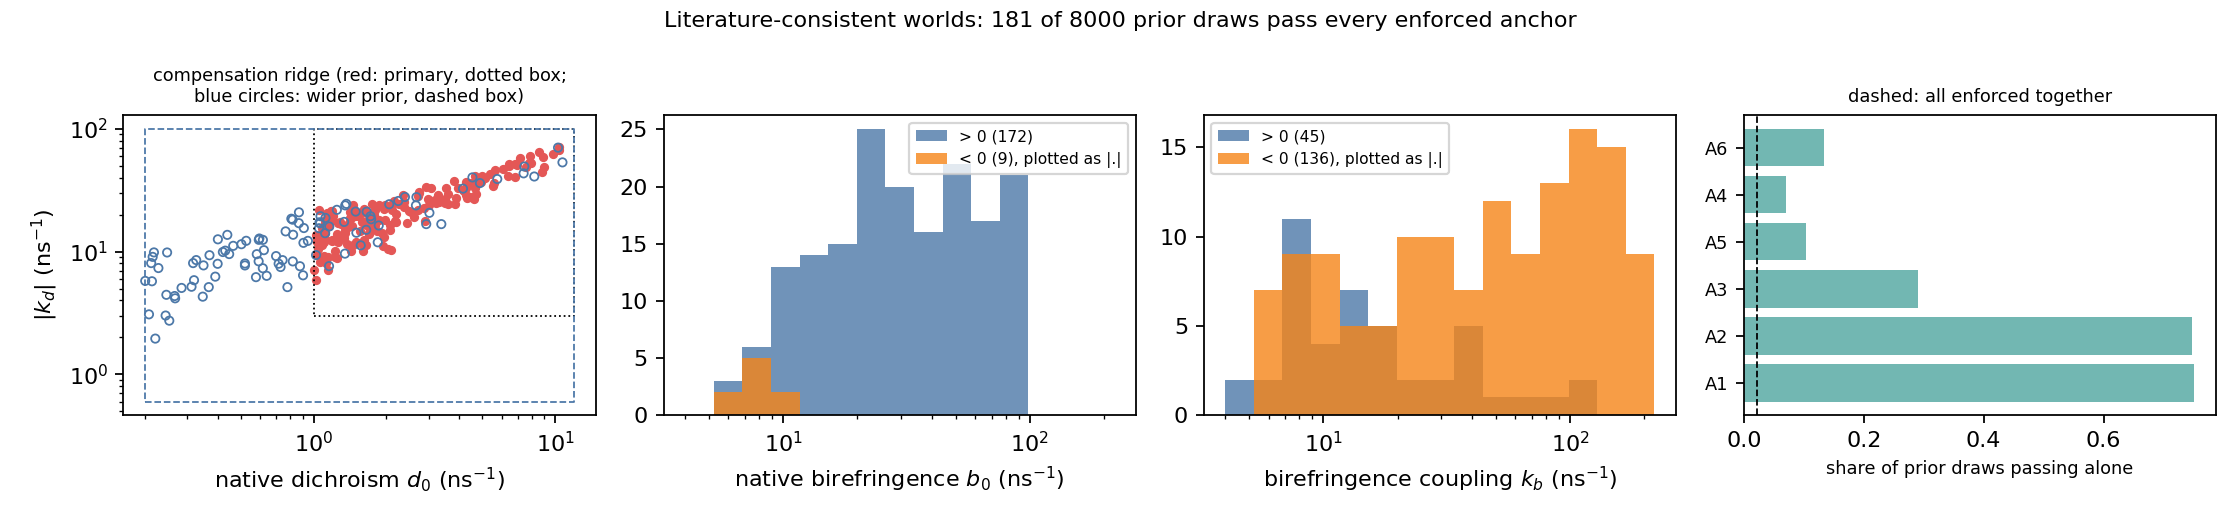
\includegraphics[width=\textwidth]{figures/anchored_worlds.png}\caption{Literature-consistent worlds. Left: native dichroism against dichroism coupling (log axes); red: primary run, dotted: its prior box; blue circles and dashed box: the run with the wider prior. Middle: native birefringence $b_0$ and birefringence coupling $k_b$ (magnitudes, split by sign). Right: share of prior draws that pass each anchor alone (dashed: all enforced anchors together).}\label{fig:anch}\end{figure}
\paragraph{The prior box matters for one constant.} The accepted native dichroism piles up against the lower edge of the prior box ($d_0\ge1$\,ns$^{-1}$): median \dzeroMedPrim{} [\dzeroQfivePrim, \dzeroQninetyfivePrim], and \dzeroNearEdgePrim\,\% of the accepted worlds lie below 2\,ns$^{-1}$. The anchors do not bound $d_0$ from below; in the model the bound comes from the device-to-device scatter of the native dichroism (0.25\,ns$^{-1}$), below which the native polarization is no longer the majority one.
A second run with the box widened to $d_0\ge0.2$ and $|k_d|\ge0.6$\,ns$^{-1}$ accepted \nAccWide{} of \nDrawsWide{} draws (\accPctWide\,\%), with median $d_0=\dzeroMedWide$\,ns$^{-1}$ and \dzeroBelowOneWide\,\% of the worlds below 1\,ns$^{-1}$. What this changes for the ranking of the design sets and for the best rotation is reported in Sec.~\ref{sec:sens}; every other result uses the primary set.
\paragraph{Two published observations are not reproduced.} (a) The $30^\circ$ cruciform is grouped with the switching devices in \cite{yuan2025apl126}; in the accepted worlds its mean switching fraction is only \pswThirty{} against \pswSixty{} ($60^\circ$) and \pswNinety{} ($90^\circ$).
(b) The symmetric cross should switch more often than the circle \cite{yuan2025clea}; here \pswSym{} against \pswCircle. Both point at the same structural limit: with a second-rank model a C$_4$ cross carries no shape anisotropy of its own, and at $30^\circ$/$60^\circ$ the
induced dichroism and birefringence vectors are not parallel to the native ones, which produces elliptical states. Predictions for angles far from $90^\circ$ should therefore be trusted least; this is a reason to measure them.

% Results sections of the supplement. Every number is a macro or table generated by scripts/make_tables.py from results/*.json.
% Every result is a MODEL PREDICTION conditional on the literature anchors of Sec. 3, not a measurement.

\section{Predicted performance of published and own designs}\label{sec:pred}
All numbers of this section are means over the \nDesignWorlds{} literature-consistent worlds (24 devices $\times$ 3 oxidation-depth nodes each); ``yield'' is the hard yield of Sec.~\ref{sec:model}.
The designs are those of the published experiments \cite{yuan2025apl126,yuan2025clea} and the 16 designs of the author's mask (families A and B, eight rotations; Sec.~\ref{sec:falsify}).
\begin{table}[H]\centering\small\tabDesigns
\caption{Predicted yield per design. The bracket gives the 10th and 90th percentile over worlds: the spread between worlds is as large as the differences between designs, so a ranking is a statement about probabilities, not about one wafer.}\label{tab:designs}\end{table}
\begin{figure}[H]\centering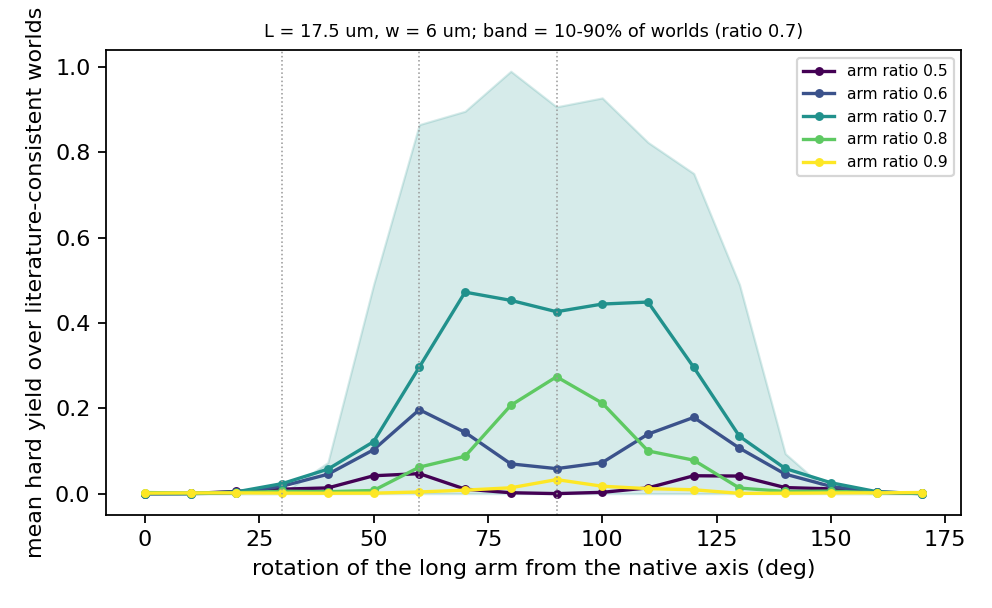
\includegraphics[width=0.62\textwidth]{figures/rotation_scan.png}\caption{Rotation scan for five arm ratios ($L=17.5\,\mu$m, $w=6\,\mu$m, $\rho=0.5$): mean hard yield over the literature-consistent worlds; the band is the 10--90\,\% range for arm ratio 0.7.}\label{fig:rot}\end{figure}
\begin{figure}[H]\centering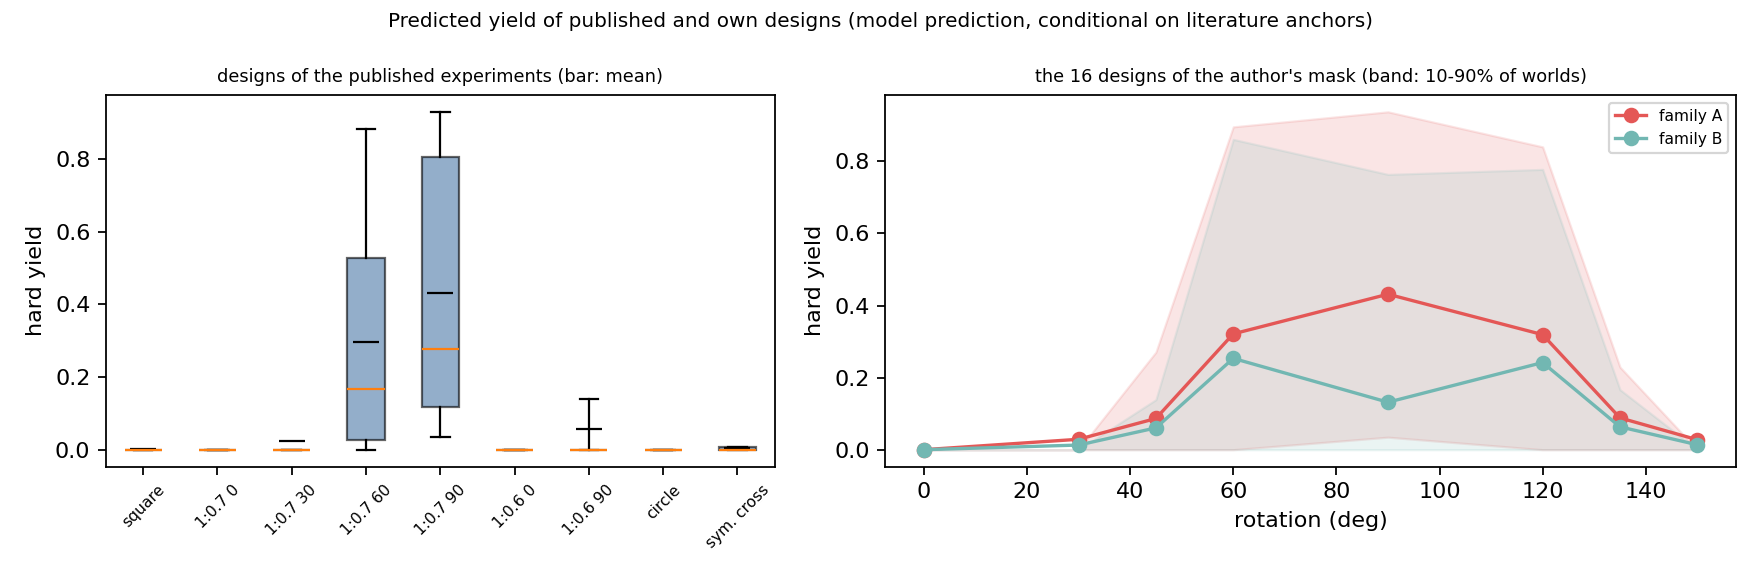
\includegraphics[width=\textwidth]{figures/designs.png}\caption{Yield of the designs of the published experiments (left) and of the 16 designs of the author's mask (right).}\label{fig:designs}\end{figure}

\paragraph{Arm ratio and rotation.} For the 1:0.7 cross the mean yield is at least 90\,\% of its maximum (\meanYieldSevenMax) for rotations between \plateauLo$^\circ$ and \plateauHi$^\circ$ (Fig.~\ref{fig:rot}); it is near zero at $0^\circ$ (long arm along the native axis, no compensation), small at $30^\circ$ and still on a steep flank at $60^\circ$.
The share of worlds in which some rotation of the cross (at $L=17.5$, $w=6$) reaches a yield of 0.5 depends strongly on the arm ratio: \reachRatioFive\,\% (0.5), \reachRatioSix\,\% (0.6), \reachRatioSeven\,\% (0.7), \reachRatioEight\,\% (0.8), \reachRatioNine\,\% (0.9).
Part of this peak at 0.7 is built into the anchors, which were formulated with the 1:0.7 and 1:0.6 designs of the experiments; it is a property of the \emph{conditional} model, not an independent confirmation that 0.7 is optimal.
\begin{table}[H]\centering\small\tabTopSeven
\caption{Among the seven designs of \cite{yuan2025apl126}: the share of worlds in which each is the best one (ties broken toward the smaller index). In \noWorkingSeven\,\% of the worlds none of the seven is a working device.}\label{tab:top7}\end{table}
\paragraph{Does the ranking of rotations depend on what counts as a good switching current?} Yes, and this matters for the answer below. The yield requires one switch inside a window of $\mu=I/I_{th}$, which is a specification of the node, not a physical constant.
Table~\ref{tab:window} scores the 1:0.7 cross at rotations from $40^\circ$ to $90^\circ$ in \nWindowWorlds{} worlds (every second literature-consistent world) under four windows.
\begin{table}[H]\centering\small\tabWindow
\caption{Mean yield of the 1:0.7 cross ($L=17.5$, $w=6\,\mu$m, $\rho=0.5$) at rotations from the native axis, for four switching-current windows (default 1.25--1.95; low bias 1.15--1.60; wide 1.15--2.05; narrow 1.50--1.70), and the share of worlds in which the $60^\circ$ device beats the $90^\circ$ one and vice versa (ties excluded).}\label{tab:window}\end{table}

\paragraph{Which aperture is best for polarization switching in an Ising node? What the evidence supports.}
\emph{Experiments} \cite{yuan2025apl126}: the text I read reports injection-locking power for the 1:0.7 cruciform rotated by $60^\circ$ (248\,$\mu$W at 10\,mA; 3.6\,$\mu$W just above threshold) and for the non-switchable square (371\,$\mu$W at 10\,mA); it does not rank all seven designs. The $30^\circ$, $60^\circ$ and $90^\circ$ cruciforms are grouped as switching devices.
That is a measurement of injection-locking power on the devices shown, not a yield, and the number of devices per design is not stated in the text I could read.
\emph{This model}, conditional on the anchors: among the designs of the published experiments only the 1:0.7 crosses at $60^\circ$ and $90^\circ$ have a substantial yield (Table~\ref{tab:designs}); the yield of a 1:0.7 cross rises steeply between $50^\circ$ and $70^\circ$, has a broad plateau between $70^\circ$ and $110^\circ$ (the mirror image of $70^\circ$--$80^\circ$ is $100^\circ$--$110^\circ$), inside which there is no reliable ranking of the rotations, and falls again beyond it. The best rotation is $70^\circ$ or $80^\circ$ in all four windows (Table~\ref{tab:window}); across the alternative ways of conditioning on the literature of Sec.~\ref{sec:sens} (Table~\ref{tab:rotsets}) the plateau is the same but its maximum moves, and $80^\circ$ (equivalently $100^\circ$) is the safest single rotation, though narrowly (Sec.~\ref{sec:sens}).
The $90^\circ$ device is close to the best rotation for the default, wide and narrow windows, but it loses about 40\,\% of its yield when switching at low bias is required, where the $60^\circ$ device is as good or better ($60^\circ$ beats $90^\circ$ in \lowBiasSixtyBeatsNinety\,\% of the worlds against \lowBiasNinetyBeatsSixty\,\% for the reverse; for the default window \defSixtyBeatsNinety\,\% against \defNinetyBeatsSixty\,\%).
This is not in conflict with the injection-locking measurement of the $60^\circ$ device, which was made just above threshold as well as at 10\,mA, but it means that ``the $60^\circ$ device was best'' and ``the $70^\circ$--$80^\circ$ device is the most robust choice'' are answers to different questions; \textbf{the mask of Sec.~\ref{sec:falsify} contains $60^\circ$, $90^\circ$ and $120^\circ$ and can inform it, but not $70^\circ$--$80^\circ$}. Restricted to the interior of the search box, the first two additions that the model would make to the mask are crosses at $70^\circ$ and $80^\circ$ (Table~\ref{tab:addint}); the first unrestricted addition is a thin-armed design at $85^\circ$ on the wall of the box.
\emph{Beyond the published designs}, the batch search of Sec.~\ref{sec:batch} favours thin-armed crosses with a small arm ratio near $85^\circ$--$90^\circ$; they lie at the edge of the search box, where the reduced model is least reliable (Sec.~\ref{sec:batch}), and are hypotheses, not recommendations.
A ranking that is meaningful for the wafer at hand requires measured constants (Sec.~\ref{sec:falsify}).

\section{Optimiser benchmark}\label{sec:bench}
\textbf{Question.} Does Bayesian optimisation find better apertures than random search, Sobol points and differential evolution for the same number of simulations (48)?
\textbf{Problems.} \emph{P1}: the wafer constants are known (one of five literature-consistent worlds), default window for the switching current ($\mu_{sw}\in[1.25,1.95]$). The five wafers were chosen among 30 accepted worlds: those in which no design of a 128-point Sobol cloud reaches a yield of 0.6 were dropped and five spanning the range of difficulty were kept, so they are not a random sample of the accepted worlds.
\emph{P2}: as P1 with a narrow window $[1.50,1.70]$ (good designs are rarer). \emph{P3}: the constants are unknown; one design is chosen to maximise the mean smoothed yield over 8 literature-consistent worlds and is scored on 24 \emph{unseen} worlds --- the situation before the first batch is measured.
\textbf{Methods.} Random search, scrambled Sobol points, differential evolution \cite{storn1997}, and Bayesian optimisation with a Gaussian-process surrogate \cite{rasmussen2006} (Mat\'ern-5/2 kernel with one length scale per input, white noise; scikit-learn \cite{pedregosa2011}; the rotation enters as $(\cos2\theta,\sin2\theta)$ so that the $180^\circ$ periodicity is exact),
with Expected Improvement \cite{jones1998} or the upper confidence bound \cite{srinivas2010,snoek2012} maximised over the design box.
\textbf{Protocol.} The optimisers see the smoothed yield on one fixed device population (common random numbers). The reported quality is the hard yield of the returned design on a \emph{fresh} population of 96 devices (and, for P3, on unseen worlds), so no method benefits from optimism about the sample it saw.
Paired Wilcoxon tests and bootstrap intervals are computed over (world, seed) pairs; \nRunsPone{} runs per method for P1 and \nRunsPthree{} for P3, 40 for P2.
\begin{table}[H]\centering\small\tabBench\caption{Mean held-out hard yield [95\,\% bootstrap interval] of the design returned by each method.}\label{tab:bench}\end{table}
\begin{table}[H]\centering\small\tabTests\caption{Paired differences (method minus baseline) of the held-out yield.}\label{tab:tests}\end{table}
\begin{figure}[H]\centering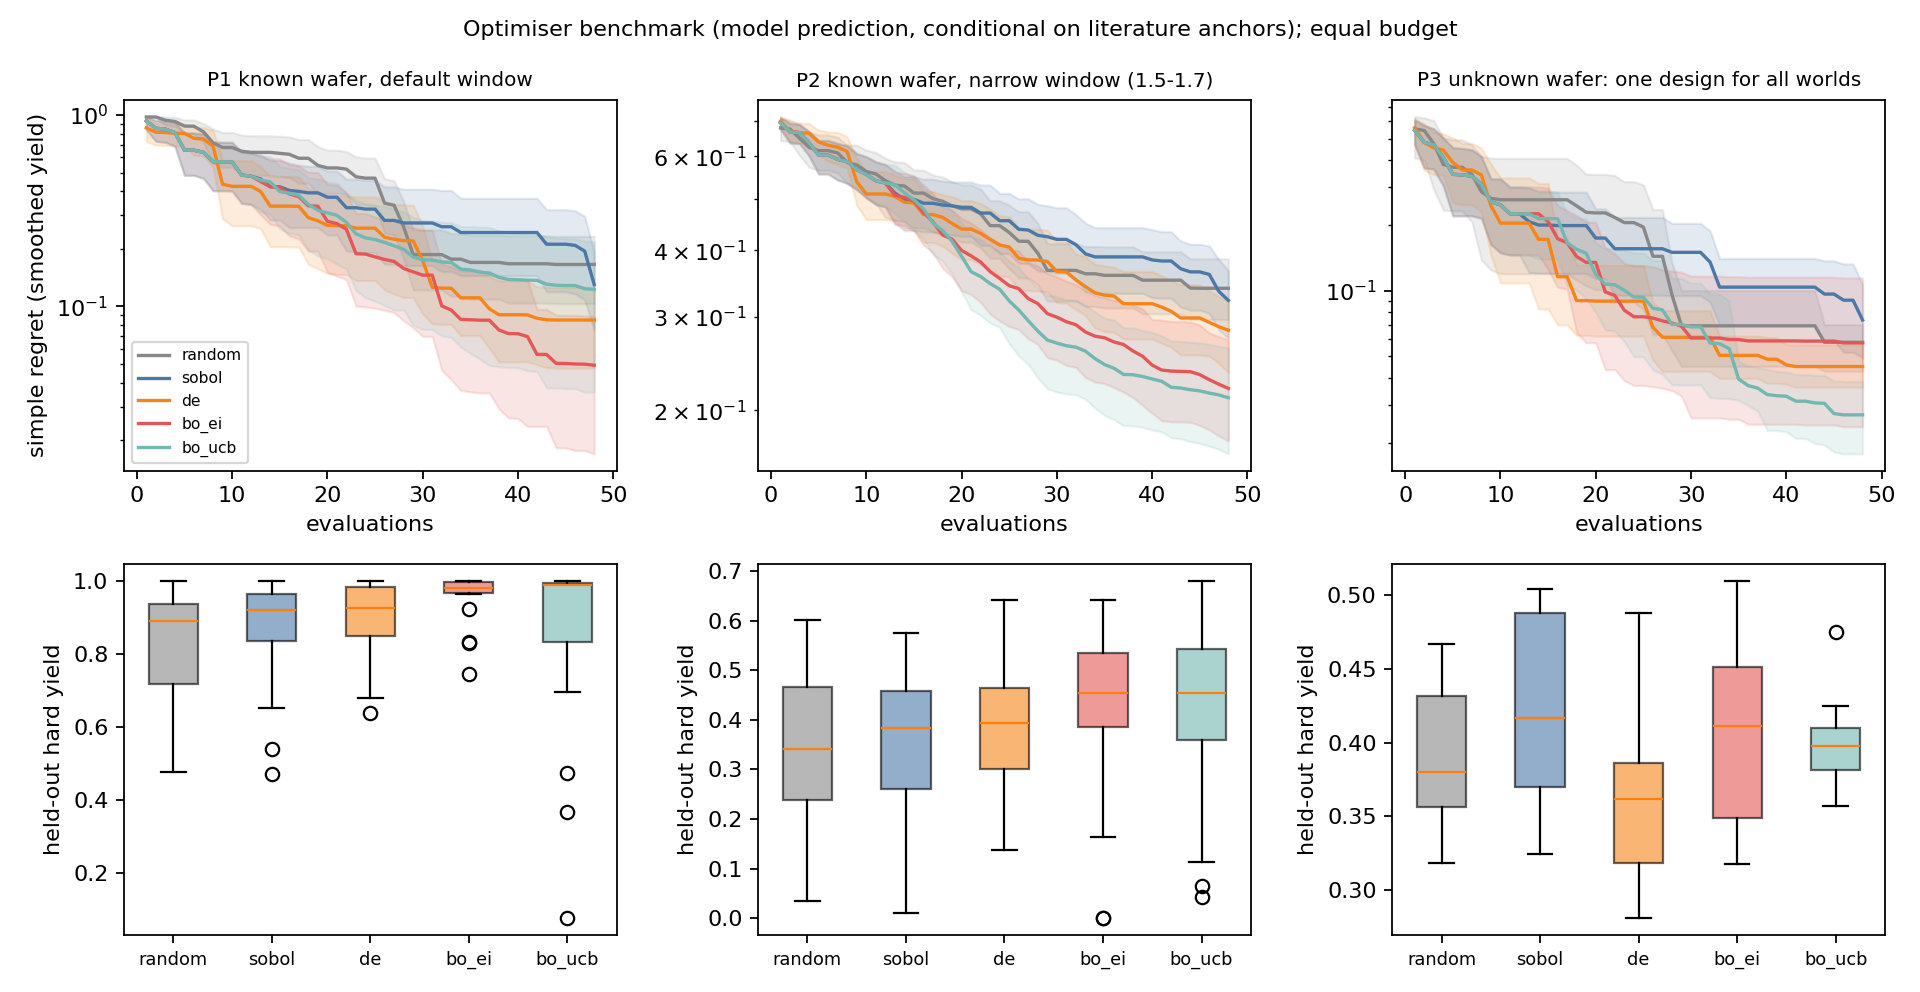
\includegraphics[width=\textwidth]{figures/benchmark.png}\caption{Top: simple regret of the smoothed yield against the best value found by any run in the same world (mean and bootstrap band). Bottom: held-out hard yield.}\label{fig:bench}\end{figure}
\paragraph{Reading of Tables~\ref{tab:bench} and~\ref{tab:tests}.}
\emph{P1 (wafer known, default window).} GP-EI returns designs with a held-out yield of \benchOneBoEi{}, against \benchOneRandom{} for random search, \benchOneSobol{} for Sobol points and \benchOneDe{} for differential evolution; all three differences are significant in paired Wilcoxon tests (\diffOneBoEiRandom{}, $p=\pvalOneBoEiRandom$; \diffOneBoEiSobol{}, $p=\pvalOneBoEiSobol$; \diffOneBoEiDe{}, $p=\pvalOneBoEiDe$; \nRunsOne{} paired runs, not corrected for six comparisons, and runs within one world are not independent).
At the level of the five wafers (the four seeds of a wafer averaged; Table~\ref{tab:wafer}) GP-EI is ahead of random search and of Sobol points on all five wafers (mean difference over wafers \waferOneBoEiRandom{} and \waferOneBoEiSobol{}, 95\,\% $t$-interval) and of differential evolution on \waferAheadOneBoEiDe{} of 5 (\waferOneBoEiDe{}); with only five wafers the interval excludes zero for random search but includes it for Sobol points (marginally) and for differential evolution.
GP-UCB is less reliable: its mean (\benchOneBoUcb{}) is not significantly above random search ($p=\pvalOneBoUcbRandom$), because \lowRunsOneBoUcb{} of its \nRunsOnePerMethod{} runs return a design with a yield below 0.5 (GP-EI: \lowRunsOneBoEi{}; random search: \lowRunsOneRandom{}).
In those runs the best value that the optimiser itself had seen on its own device population was also low (\ucbLowBestMin--\ucbLowBestMax), so they had not converged within 48 evaluations (the fixed exploration weight $\beta=2$ is the likely reason; I did not test other weights) rather than over-fitted the population.
\emph{P2 (wafer known, narrow window).} Both Bayesian optimisers return designs with a held-out yield of \benchTwoBoEi{} (GP-EI) and \benchTwoBoUcb{} (GP-UCB), against \benchTwoRandom{} for random search, \benchTwoSobol{} for Sobol points and \benchTwoDe{} for differential evolution.
The gain over random search (\diffTwoBoEiRandom{}, $p=\pvalTwoBoEiRandom$) and over Sobol points (\diffTwoBoEiSobol{}, $p=\pvalTwoBoEiSobol$) is significant in paired Wilcoxon tests (not corrected for six comparisons; the GP-UCB values are in Table~\ref{tab:tests});
the gain over differential evolution (\diffTwoBoEiDe{}, $p=\pvalTwoBoEiDe$ for GP-EI; \diffTwoBoUcbDe{}, $p=\pvalTwoBoUcbDe$ for GP-UCB) is not.
By world, the better Bayesian optimiser leads differential evolution by more than 0.02 in \worldsBoAheadDeTwo{} of the \nWorldsTwo{} worlds, is level in \worldsTieBoDeTwo{} and trails in \worldsDeAheadBoTwo{}; the eight seeds of one world are not independent draws of the problem, so the tests overstate the effective sample size.
At the level of wafers (Table~\ref{tab:wafer}) GP-EI is ahead of random search on \waferAheadTwoBoEiRandom{} and of Sobol points on \waferAheadTwoBoEiSobol{} of 5 wafers, GP-UCB on \waferAheadTwoBoUcbRandom{} and \waferAheadTwoBoUcbSobol{}; the interval over wafers excludes zero for GP-EI against random search and for GP-UCB against random search and Sobol points, and includes it in every comparison with differential evolution.
\begin{table}[H]\centering\small\tabWafer\caption{Optimiser benchmark at the level of wafers: the seeds of a wafer are averaged and the five wafer means are compared (mean difference of the held-out yield, 95\,\% $t$-interval over wafers, number of wafers in which the Bayesian optimiser is ahead).}\label{tab:wafer}\end{table}
\emph{P3 (wafer unknown; one design for eight worlds, scored on 24 unseen worlds).} The five methods lie between \benchThreeMin{} and \benchThreeMax{} and no difference is significant (Friedman test over the five methods, $p=\friedThree$; \nRunsThree{} runs per method, so differences of a few hundredths could not be detected).
All five methods lose about the same amount between the eight selection worlds (\pThreeSelLo--\pThreeSelHi, the yield of the returned design on those worlds) and the 24 unseen ones (\pThreeUnseenLo--\pThreeUnseenHi; a loss of \pThreeGapLo--\pThreeGapHi): a design tuned on eight worlds mostly over-fits them, whichever search algorithm produced it, and with eight runs per method the test has little power.
This is the situation that motivates the batch of Sec.~\ref{sec:batch}, whose score is a different quantity: the expected best-of-batch yield (0.86 on 32 unseen worlds, \othPortOther{} on \nOtherWorlds{} further ones) assumes that the best design of the batch can be identified after measurement and is not comparable with the yield of one design.
P3 does not show that a single design cannot hedge: the best single design of the pool, chosen on 32 training worlds, reaches \singleBestYield{} on 32 other worlds (Table~\ref{tab:batch}), although it lies on a wall of the search box.
\emph{What this does not show.} A simulator evaluation costs a fraction of a second, so the budget of 48 is a statement about sample efficiency, not about cost; a fabrication run is many orders of magnitude more expensive and the real batch is 16 designs.
The optimiser and the scoring use the same reduced model, so the benchmark says nothing about how well the model represents devices.

\section{Designing a fabrication batch}\label{sec:batch}
A mask is a batch: the 16 designs are fixed before any measurement, and the constants of the wafer are still unknown. The batch is therefore chosen to maximise the \emph{expected best yield in the batch},
$E_w[\max_j Y_j(w)]$ over worlds $w$, a monotone submodular set function that a greedy algorithm maximises within a factor $1-1/e$ of the optimum \cite{nemhauser1978}.
\textbf{Candidates:} \nPool{} designs (128 Sobol points; the best designs of two prior-robust Bayesian-optimisation runs; the nine reference designs; the author's 16; a rotation family). \textbf{Selection:} on \nTrainWorlds{} \emph{training} worlds only.
\textbf{Scoring:} on \nTestWorlds{} disjoint \emph{test} worlds (all worlds are literature-consistent, so the test worlds share the assumptions of the training worlds; they are unseen constants, not an independent check of the model).
This is not the batch Bayesian optimisation of \cite{desautels2014}, which spreads a batch over a Gaussian-process posterior; that alternative was not compared.
\begin{table}[H]\centering\small\tabBatch\caption{Expected best-of-batch yield on unseen worlds. In \noWorkingTest{} of the \nTestWorlds{} test worlds no design of the pool reaches a yield of 0.3.}\label{tab:batch}\end{table}
\begin{table}[H]\centering\small\tabMaskPlus\caption{Adding $k$ designs (chosen on the training worlds) to the author's 16-design mask.}\label{tab:maskplus}\end{table}
\begin{table}[H]\centering\small\tabAdd\caption{The added designs of Table~\ref{tab:maskplus}, in the order of the greedy choice.}\label{tab:add}\end{table}
\begin{table}[H]\centering\small\tabBatchList\caption{The 16 designs of the portfolio (lengths in $\mu$m, $\rho$ = corner rounding, $\theta$ = rotation in degrees), with their yield on training and test worlds.}\label{tab:batchlist}\end{table}
\begin{figure}[H]\centering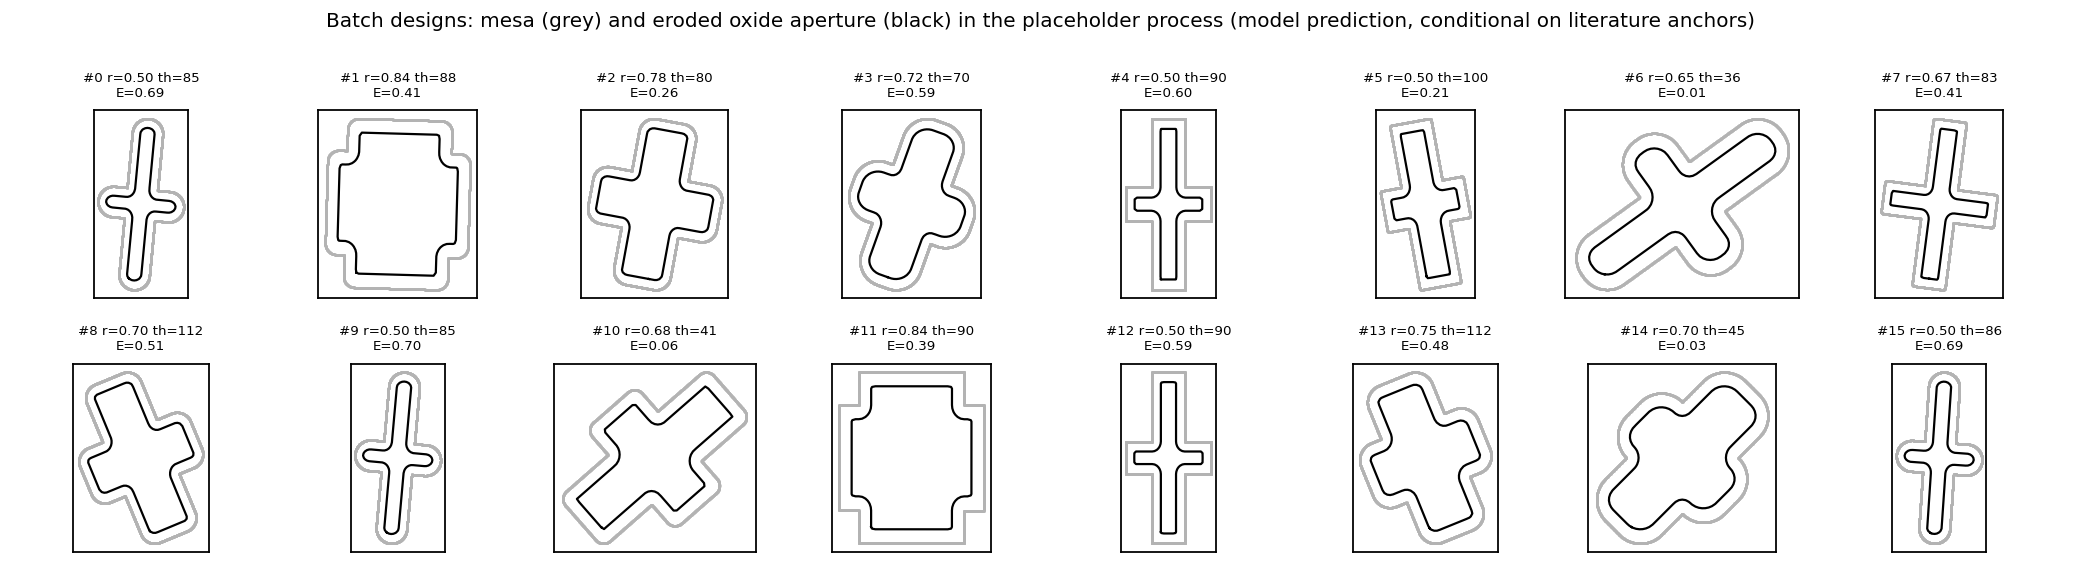
\includegraphics[width=\textwidth]{figures/batch_shapes.png}\caption{The portfolio: mesa (grey) and eroded oxide aperture (black) in the placeholder process.}\label{fig:batch}\end{figure}
\paragraph{Boundary and fresh-device checks.} \nWall{} of the \nQ{} portfolio designs sit on a wall of the search box (thinnest arms and/or lowest arm ratio); their oxide apertures have an area of only \wallAreaLo--\wallAreaHi\,$\mu$m$^2$
against \refAreaLo--\refAreaHi\,$\mu$m$^2$ for the cruciforms of the experiments and \circleArea\,$\mu$m$^2$ for the circle (Table~\ref{tab:walls}). Thin arms are where the scalar-mode, single-mode description is least credible and where loss and current density that the model does not contain would matter.
Two checks were made on the same test worlds: (i) the sets were re-scored on a new population of \freshDev{} devices, so that the comparison cannot come from over-fitting to particular device draws; (ii) a portfolio was re-selected from the \nPoolInterior{} candidates of the pool inside a conservative interior box (arm ratio $\ge0.6$, $4.5\le w\le7.5\,\mu$m, $13\le L\le19\,\mu$m).
\begin{table}[H]\centering\small\tabInterior\caption{Fresh device population; same unseen worlds.}\label{tab:interior}\end{table}
\begin{table}[H]\centering\small\tabWalls\caption{Portfolio designs with the area of their oxide aperture in the placeholder process.}\label{tab:walls}\end{table}
The advantage of the model-selected batch over the author's mask and over the seven published designs survives both checks (Table~\ref{tab:interior}); the interior-only batch gives up part of it (\interiorSame{} on the original devices), which is the price of staying where the model is credible.
\paragraph{What the batch tells the author about her mask.} Most of the value comes from a few designs: the first four designs of the greedy order already reach 0.81 on the training worlds and the first eight give nearly the same expected best yield on the test worlds as all sixteen (0.85 against 0.86; Table~\ref{tab:batch}).
Adding designs to the author's mask helps nearly as much as replacing it: Table~\ref{tab:maskplus} shows that two additions lift the expected best yield from 0.68 to about 0.85, close to the level of the whole portfolio, but the first of them is a thin-armed design on the wall of the search box, so it is a hypothesis rather than a recommendation.
Restricting the additions to the interior box (Table~\ref{tab:addint}) gives \intPlusOne{} with one added design, \intPlusTwo{} with two and \intPlusThree{} with three, about the level of the interior-only sixteen-design portfolio (Table~\ref{tab:interior}), and the first two additions are crosses close to mask family~A (arm ratio 0.72--0.78, width about 6.2--6.3\,$\mu$m) at $70^\circ$ and $80^\circ$, rotations that the mask does not contain.
The mask's rotations come in mirror pairs ($30^\circ$/$150^\circ$, $45^\circ$/$135^\circ$, $60^\circ$/$120^\circ$), which the model treats as equivalent up to device scatter: the pairs are replicates and a test of the mirror symmetry of the wafer (a difference between a design and its twin could point to strain, an off-cut substrate or misalignment), but they also mean that the mask samples only five distinct rotations.
\begin{table}[H]\centering\small\tabAddInterior\caption{Additions to the author's mask restricted to the interior box, in the order of the greedy choice (chosen on the training worlds, scored on the test worlds).}\label{tab:addint}\end{table}
\paragraph{How optimistic is the headline?} The \nTestWorlds{} test worlds were never used to choose the portfolio, but they are only \nTestWorlds{} of the \nAccepted{} accepted worlds. Scoring the same sets on the \nOtherWorlds{} accepted worlds that were used neither for selection nor for this test (same devices, same specification) gives lower levels and the same ordering (Table~\ref{tab:other}): portfolio \othPortOther{}, author's mask \othMaskOther{}, seven published designs \othSevenOther{}; portfolio minus mask \othDiffPortMaskOther{} (95\,\% bootstrap interval over worlds).
The mask with three interior additions reaches \othMaskIntOther{} on these worlds (\intPlusThree{} on the test worlds). The 0.86 is therefore an optimistic draw of 32 worlds; the level to quote is about \othPortNon{} (all \nNontrainWorlds{} worlds not used for selection), and it assumes that the best design of the batch can be identified after measurement.
\begin{table}[H]\centering\small\tabOther\caption{Expected best-of-batch yield on three sets of accepted worlds, none used to select the designs (\texttt{scripts/other\_worlds\_check.py}).}\label{tab:other}\end{table}

\section{Sensitivity to the assumptions}\label{sec:sens}
Each row perturbs the model or re-conditions it on the literature, and re-scores three sets of designs: the portfolio, the author's mask and the seven designs of \cite{yuan2025apl126}. What matters is the \emph{order} of the sets, not the absolute level. The portfolio was selected once, under the baseline assumptions.
The first rows keep the 32 test worlds and change one assumption. The rows from ``worlds accepted with LOOSE thresholds'' on use 32 newly accepted worlds: under another translation of the anchors into thresholds (loose, strict; Sec.~\ref{sec:anchor}), under the wider prior of Sec.~\ref{sec:anchor}, or (``RECONDITIONED'') after an assumption was changed \emph{and} the four constants were re-inferred from the same literature outcomes (4000 prior draws each).
The spin-flip constants of \cite{chen2026meta} accept no world (\nAccChen{} of \nDrawsChen{} draws), so for them only the row with the old worlds exists.
\begin{table}[H]\centering\scriptsize\tabSens\caption{Expected best-of-batch yield under perturbations (32 worlds per row).}\label{tab:sens}\end{table}
\paragraph{Reading of Table~\ref{tab:sens}.} The ordering portfolio $>$ mask $>$ seven published designs holds in \sensOk{} of \sensN{} rows (the baseline is one of the rows, and in the row with the spin-flip constants of \cite{chen2026meta} no set switches at all), but the rows are not equally informative; the absolute level is not stable at all (the portfolio's expected best yield runs from \sensPortMin{} to \sensPortMax{}).
\emph{Robust (baseline and 14 rows).} Oxidation depth 0.7 and 1.3\,$\mu$m, oxidation-rate ratio 1.3 (also when the constants are re-inferred), index step, device scatter, mask tolerance, finer geometry grid, the low-bias and the wide switching-current windows, loose and strict thresholds and the wider prior keep the portfolio ahead of the mask by 0.05--0.28 at an expected best yield of 0.68--0.92.
\emph{Ordering fails without re-inferring the constants (5 rows).} Isotropic oxidation ($\eta=1.0$): mask 0.82, seven designs 0.77, portfolio 0.75. Half the coupling constants: seven 0.67, mask 0.43, portfolio 0.25. Thermal dichroism drift of $|\chi_{th}|=0.2$: all three sets between 0.04 and 0.27. The spin-flip constants of \cite{chen2026meta} with the old worlds: no device switches in any set.
These rows move a constant away from the values that reproduce the literature (halving the coupling, for instance, breaks the cancellation of the native dichroism at arm ratio 0.7, the ridge of Fig.~\ref{fig:anch}); the world is then no longer literature-consistent, so a low yield shows how tightly the design is tied to that ridge, not that the literature contradicts it.
\emph{Ordering holds only weakly or at low yields (3 rows).} $\chi_{th}=-0.05$ (0.72, 0.70, 0.69: indistinguishable), $\chi_{th}=+0.05$ (0.29, 0.18, 0.13), coupling $\times2$ (0.39, 0.25, 0.20).
\paragraph{Re-conditioned rows: what depends on the assumption itself.}
\emph{Oxidation.} With isotropic oxidation, \nAccOxTen{} of \nDrawsOxTen{} draws still reproduce the literature outcomes, but the portfolio and the mask tie (0.61 each; seven designs 0.56): the advantage of a model-selected batch over the mask depends on the anisotropy of the oxidation. With $\eta=1.3$ (\nAccOxThirteen{} accepted) it remains (0.77 against 0.71). The oxide anisotropy is measurable on a cross-section or an infrared image of the oxide front, far more cheaply than a mask run.
\emph{Thermal drift.} With $\chi_{th}=\pm0.2$ (a dichroism that moves with current by an amount comparable to the native one across the operating range; the scale is an arbitrary probe, not an estimate) the literature outcomes are still reproduced (\nAccChiMinus{} and \nAccChiPlus{} worlds accepted), but no set of designs exceeds an expected best yield of 0.24 and the ordering is lost or meaningless (0.17, 0.24, 0.11 for $-0.2$; 0.09, 0.07, 0.03 for $+0.2$).
The sign of the native birefringence also follows the sign of $\chi_{th}$: $b_0>0$ in \fracBzeroPosChiMinus{}\,\% of the accepted worlds for $\chi_{th}=-0.2$ and in \fracBzeroPosChiPlus{}\,\% for $+0.2$, against \fracBzeroPos{}\,\% in the primary set.
The ``$b_0>0$'' of Sec.~\ref{sec:anchor} is therefore a consequence of assuming no thermal drift, not something the literature fixes, and \textbf{every yield in this study presumes that the switching comes from the spin-flip dynamics at a fixed anisotropy}. If the switching of the fabricated devices is thermally driven, these predictions do not apply.
\emph{Wider prior.} With native dichroism allowed down to 0.2\,ns$^{-1}$ the portfolio still leads the mask, but by 0.09 (0.72 against 0.63, the seven designs 0.63).
\paragraph{Does the best rotation depend on how the literature was translated into constraints?}
The 1:0.7 cross ($L=17.5$, $w=6\,\mu$m, $\rho=0.5$) was scored at eleven rotations on the worlds of every conditioning above (Table~\ref{tab:rotsets}; at most 40 worlds per set, the constants of \cite{chen2026meta} accept no world).
\begin{table}[H]\centering\scriptsize\resizebox{\textwidth}{!}{\tabRotSets}\caption{Mean hard yield of the 1:0.7 cross by rotation from the native axis, in each set of worlds; last row: for each rotation the lowest share of the set's own best rotation among the \nRotWorking{} sets in which some rotation works (best mean yield $\ge0.2$). $\theta$ and $180^\circ-\theta$ are mirror images; a ``best'' of $70^\circ$ or $110^\circ$ is the same statement.}\label{tab:rotsets}\end{table}
In the \nRotWorking{} working sets the yield forms the same plateau between $70^\circ$ and $110^\circ$ (approximately mirror-symmetric about $90^\circ$), and it is only \shareSixtyLo--\shareSixtyHi\,\% of the set's best at $60^\circ$ and \shareOneTwentyLo--\shareOneTwentyHi\,\% at $120^\circ$.
Where the maximum lies inside the plateau does depend on the set: $70^\circ$/$110^\circ$ in the primary and loose sets, $80^\circ$--$100^\circ$ in the strict, wider-prior and $\eta=1.3$ sets, $90^\circ$ with isotropic oxidation.
Measured against the best rotation of each set, $80^\circ$ (and its mirror image, $100^\circ$) never falls below \rotWorstEightZero{} of that set's best, $90^\circ$ below \rotWorstNineZero{} and $70^\circ$/$110^\circ$ below \rotWorstSevenZero{}.
\textbf{In this model $80^\circ$ (equivalently $100^\circ$) is the most robust single rotation, narrowly}, and there is no reliable ranking inside the $70^\circ$--$110^\circ$ plateau: these are point estimates from 40 worlds per set. Resampling the worlds (\nBootRot{} bootstrap resamples, yields averaged with the mirror-image rotation) gives $80^\circ$ the highest worst case in \pHighestEighty\,\% of the resamples ($90^\circ$: \pHighestNinety\,\%, $70^\circ$: \pHighestSeventy\,\%), $80^\circ$ above $90^\circ$ in \pEightyAboveNinety\,\% and above $70^\circ$ in \pEightyAboveSeventy\,\%; the worst-case share is \worstMeanEighty{} (95\,\% interval \worstLoEighty--\worstHiEighty) at $80^\circ$, \worstMeanNinety{} (\worstLoNinety--\worstHiNinety) at $90^\circ$ and \worstMeanSeventy{} (\worstLoSeventy--\worstHiSeventy) at $70^\circ$. The preference for $80^\circ$ over $90^\circ$ is therefore indicative, not established; the firm statement is that $80^\circ$--$100^\circ$ is the core of the plateau, and the statement of Sec.~\ref{sec:pred} that $70^\circ$--$80^\circ$ is best is a statement about the primary set.
With thermal drift (last two sets) no rotation works (best mean yield 0.05 or lower), so no rotation can be recommended if switching is thermally driven.
\paragraph{What to measure first.} The rows above point at the same three unknowns, in the order of their leverage on the design: (1) the anisotropy and depth of the oxidation (cross-sections, infrared images of the oxide front); (2) whether the switching of a fabricated device follows the current or the temperature (polarization-resolved $L$--$I$ curves at several heat-sink temperatures); (3) the scale of the birefringence and dichroism that a given shape produces (polarization-resolved spectra below threshold, as in \cite{choquette1995}).

\subsection{Is the birefringence channel optical or mechanical? A semi-vectorial check}\label{sec:formbiref}
The model routes the shape dependence of the birefringence through a stress-weighted boundary tensor with a free coefficient $k_b$ (Sec.~\ref{sec:model}). One part of the birefringence can instead be computed without free coefficients: the \emph{form} birefringence of the lateral index guide that the aperture defines. A semi-vectorial finite-difference solver (\texttt{src/vcsel\_bo/vector\_modes.py}) solves the transverse equation for each linear polarization, with the normal component $\varepsilon E_\perp$ continuous across index steps, on the same grid for both polarizations; solving on grids aligned with $0^\circ$ and $45^\circ$ gives the magnitude and axis of the splitting, converted as $\Delta\nu=\nu\,\Delta n_{\mathrm{eff}}/n_g$ and $\gamma_p=\pi\Delta\nu$ ($n_g=3.6$ and index step $\Delta n_{\mathrm{eff}}=0.01$ assumed).
\emph{Checks.} The solver reproduces the exact TE--TM splitting of a dielectric slab to 0.1\,\% (second-order convergence), gives no splitting for a circle, follows the long axis of an ellipse under rotation, and changes by \(1.3\,\%\) between grids of 0.1 and 0.07\,$\mu$m.
\begin{table}[H]\centering\small
\begin{tabular}{lrrrrr}\toprule
Design & $\Delta n_{\mathrm{eff}}$ ($10^{-6}$) & axis ($^\circ$) & split.\ (MHz) & $\gamma_p^{\mathrm{form}}$ (ns$^{-1}$) & $|k_b||\mathbf s_{stress}|$ (ns$^{-1}$) [5--95\,\%]\\\midrule
A0 & 0.26 & 0.2 & 23 & 0.07 & 6.7 [1.2--32.9]\\
A60 & 0.33 & 61.6 & 29 & 0.09 & 6.8 [1.2--33.2]\\
A90 & 0.36 & 89.9 & 31 & 0.10 & 6.9 [1.2--33.5]\\
B0 & 0.51 & 0.1 & 46 & 0.14 & 9.8 [1.8--48.0]\\
B60 & 0.52 & 59.5 & 46 & 0.15 & 9.3 [1.7--45.5]\\
B90 & 0.53 & 89.9 & 47 & 0.15 & 9.1 [1.7--44.6]\\\bottomrule
\end{tabular}
\caption{Form birefringence of six designs of the author's mask (placeholder process: depth $1\,\mu$m, oxidation-rate ratio 1.15; all 16 designs and the isotropic process are in \texttt{results/form\_birefringence.json}), compared with the phenomenological stress term over the literature-consistent worlds. MODEL PREDICTIONS.}\label{tab:formbiref}\end{table}
\paragraph{Reading.} Over all 16 designs the form birefringence is 0.07--0.15\,ns$^{-1}$ (splittings of 20--50\,MHz); with a five times larger index step (0.05) it stays at or below 0.4\,ns$^{-1}$. Measured VCSEL splittings are 1.3--9.9\,GHz ($\gamma_p\approx4$--31\,ns$^{-1}$, \cite{choquette1995}), and the stress term needed to reproduce the published outcomes is of the same order. The shape therefore acts on the birefringence mainly through strain, not through the optics of the guide, which supports routing it through a stress channel; but the $1/(r^2+1)$ kernel of that channel remains an assumption. The next simulation of value is a mechanical one (oxide shrinkage as the load, then the photoelastic tensor of GaAs), not a more accurate optical solver. The sign with which the form term would enter the SFM depends on the field-envelope convention and was not verified; the term is too small to change the results either way.

\section{Testable predictions for the mask}\label{sec:falsify}
The mask has two aperture families (A: $17.5\times12.25\,\mu$m, corners assumed sharp; B: $15.0\times10.5\,\mu$m, short-arm radius $2.25\,\mu$m; arm width $6\,\mu$m) at eight rotations, 32 devices in all, i.e.\ two per design if all designs are equally represented.
Table~\ref{tab:maskpred} lists what the \nMaskWorlds{} literature-consistent worlds predict; the median and the 10--90\,\% interval over worlds are given, because the constants are not known.
\begin{table}[H]\centering\small\resizebox{\textwidth}{!}{\tabMaskPred}\caption{Predictions for the 16 designs of the mask (rotation from the native axis $x$). Azimuth of the low-current state in the crystal frame: axial mean over worlds (0$^\circ$ and 180$^\circ$ are the same direction) with the resultant length $R$ in brackets ($R$ near 1: the worlds agree; near 0: they do not).}\label{tab:maskpred}\end{table}
\begin{table}[H]\centering\small\tabOrder\caption{Pairwise orderings of yield across worlds.}\label{tab:order}\end{table}
\paragraph{Predicted numbers of switching devices (two devices per design).} Drawing a world and then two Bernoulli devices per design, the model predicts for the 12 devices of the $60^\circ$, $90^\circ$, $120^\circ$ designs a mean of \cntHighMean{} switching devices (5th--95th percentile: \cntHighLo--\cntHighHi), for the \cntNearZeroN{} devices at $0^\circ$, $30^\circ$, $150^\circ$ a mean of \cntNearZeroMean{} (\cntNearZeroLo--\cntNearZeroHi), and for the \cntMidN{} devices at $45^\circ$, $135^\circ$ a mean of \cntMidMean{} (\cntMidLo--\cntMidHi).
If the arm tips of family A were fully rounded ($\rho=\rhoFamilyA$) instead of sharp, the means become \cntHighRoundMean{} (\cntHighRoundLo--\cntHighRoundHi) at $60^\circ$--$120^\circ$, \cntNearZeroRoundMean{} near $0^\circ$ and \cntMidRoundMean{} at $45^\circ$, $135^\circ$ (\texttt{scripts/mask\_family\_a\_rounded.py}): the corner treatment shifts the numbers a little but does not change the picture.
Here a device \emph{switches} if it shows at least one polarization flip in the sweep; the number of devices that also meet the whole yield specification (one switch inside the current window, stable states, separation, ellipticity) is smaller: \cntHighPassMean{} of the 12 devices at $60^\circ$--$120^\circ$ (\cntHighPassLo--\cntHighPassHi) and \cntNearZeroPassMean{} of the \cntNearZeroN{} near $0^\circ$.
\textbf{How the predictions can fail.} A measurement outside these intervals --- more than \cntNearZeroHi{} of the \cntNearZeroN{} devices near $0^\circ$ switching, or none of the 12 devices at $60^\circ$--$120^\circ$ --- lies beyond the 5th or 95th percentile of the prediction, so it would count against the model class at about the 5\,\% level for each statement; it would not by itself refute it, because the placeholder oxidation, the two devices per design and the assumed sharp corners of family A could equally be at fault. The near-$0^\circ$ group contains the $30^\circ$ and $150^\circ$ designs, and switching of the $30^\circ$ cross is a published observation that the model does not reproduce (Sec.~\ref{sec:anchor}), so a switching $30^\circ$ device would not be a new failure.
The intervals are wide because the literature-consistent set is wide; with the first measurement they are expected to narrow, not to close.
Design-level statements are weaker still: with two devices, one design cannot distinguish a yield of 0.3 from 0.7. Measuring at least eight devices for the four designs $60^\circ$ and $90^\circ$ of family A and B would be a natural extension (the author's judgement, not a computed optimum).
Further qualitative predictions: in the median world the low-current polarization follows the long arm ($x$ for $0^\circ$--$30^\circ$, $y$ for $60^\circ$--$120^\circ$), but family A at $60^\circ$ and $120^\circ$ lases first on $x$ in \xLikeAsixty\,\% and \xLikeAonetwenty\,\% of the worlds (family B: \xLikeBsixty\,\% and \xLikeBonetwenty\,\%), so this is a probabilistic prediction; mirror-image rotations ($\theta$ and $180^\circ-\theta$) behave alike within scatter (Table~\ref{tab:order}: e.g.\ $30^\circ$ against $150^\circ$).
\paragraph{Calibration protocol.} For every fabricated design record, from polarization-resolved $L$--$I$ sweeps ($1.05$--$2.1\,I_{th}$, fixed temperature): the number of devices $n$, the number with exactly one polarization switch, the median switching current $\mu_{sw}$ of the switchers, and the azimuth of the low-current state in the crystal frame ($x$ = wafer flat).
Then \texttt{vcsel\_bo.calibration.abc\_posterior(observations, worlds=...)} re-weights the literature-consistent worlds by how well their simulated summaries reproduce the measured ones (Gaussian-kernel ABC \cite{beaumont2002}); the batch design of Sec.~\ref{sec:batch} is re-run on the posterior worlds. The module is exercised on synthetic data only (\texttt{tests/test\_calibration.py}).
\paragraph{What could a first batch teach? (synthetic test, well specified, therefore optimistic).} The wafer is assumed to be one of \voiNWorlds{} literature-consistent worlds; the mask is ``measured'' with $n$ devices per design; the other worlds are re-weighted by the likelihood of the counts (and, in a second model, of the azimuth and switching current); the pool design with the largest posterior expected yield is chosen and scored in the true world.
Without any measurement the best single design of the pool has a mean yield of \voiNone{}; the oracle that knows the true world reaches \voiOracle{}.
\begin{table}[H]\centering\small\resizebox{\textwidth}{!}{\tabVOI}\caption{A synthetic first batch. Yield of the design chosen after the measurement (no measurement: \voiNone; oracle: \voiOracle). Prior probability of the correct sign of $k_b$ from the base rate: \voiPriorSign.}\label{tab:voi}\end{table}
The gain is modest --- from \voiNone{} to \voiLo--\voiHi{} --- and does not grow with more devices per design, because the posterior collapses onto very few of the \voiNWorlds{} worlds (effective sample size \voiEssLo--\voiEssHi); tempering the likelihood does not change this. The sign of the birefringence coupling $k_b$, which the literature leaves open, is recovered with a probability of at most \voiSignHi{}, against \voiPriorSign{} for always guessing the more frequent sign.
Two lessons: a continuous calibration model rather than a finite set of worlds is needed once measurements exist, and the azimuth of the low-current state and the switching current should be recorded, not only whether a device switches.

% \section{Open questions where machine-learning theory would help (not implemented)}\label{sec:open}
% \begin{itemize}\setlength\itemsep{1pt}
% \item \textbf{Comparing simulated and measured device populations.} The anchors are hand-made summaries with hand-made tolerances. A distance between the two \emph{distributions} of devices --- the maximum mean discrepancy \cite{gretton2012}, or a Wasserstein distance as in \cite{bernton2019} --- and a robust posterior that tolerates a misspecified simulator \cite{cheriefabdellatif2020} would replace both.
% \item \textbf{Sampling efficiency.} The rejection sampler accepts \accPct\,\% of its draws; a sequential Monte Carlo sampler for approximate Bayesian computation \cite{delmoral2012} is the obvious remedy.
% \item \textbf{From simulator to wafer.} The fabricated wafer is a different domain from the simulator; learning across domains \cite{bendavid2010} asks under which conditions a design chosen in the first transfers to the second, and what a handful of measured devices can guarantee.
% \item \textbf{Batches on the surrogate.} Methods that spread a batch over a Gaussian-process posterior \cite{desautels2014} should be compared with the portfolio design used here.
% \end{itemize}


\section{Limitations and what remains uncertain}
\begin{itemize}\setlength\itemsep{1pt}
\item Constants and process parameters are not measured; the anchors are qualitative and many worlds satisfy them. Conclusions are therefore stated as distributions over worlds, never as one fitted value.
\item Thresholds that translate ``most/seldom/part'' into numbers are choices (Sec.~\ref{sec:sens} shows their effect); the sizes of the fabricated apertures are not in the text read, so the published designs are drawn at assumed sizes ($L=17.5\,\mu$m, $w=6\,\mu$m, corner fraction 0.5).
\item Structural limits: single-mode SFM although apertures of this size may be multimode; scalar mode used only as a weight; linear phenomenological coupling; second-rank symmetry; the birefringence channel is attributed to stress, which a semi-vectorial check supports only indirectly (the optical form birefringence is 25--450 times smaller than measured splittings at the assumed index step, and at least 10 times smaller at a five times larger step, Sec.~\ref{sec:formbiref}) and which no mechanical simulation has computed; two of six published observations not reproduced (Sec.~\ref{sec:anchor}).
\item Sources not read in full: \cite{yuan2025jlt} (abstract only), \cite{yuan2025apl127} (listing only). The SFM constants of \cite{yuan2025apl126} could not be re-checked in the last pass; the model uses typical magnitudes. The second set, from \cite{chen2026meta} (spin-flip rate 20 times larger), accepts no world in 4000 draws, so that robustness check is inconclusive, not confirmatory.
\item The corner treatment of mask family A is not recorded in the project notes and is assumed sharp; family B has the recorded $2.25\,\mu$m short-arm radius. With fully rounded arm tips for family A the predicted number of switching devices at $60^\circ$--$120^\circ$ falls from \cntHighMean{} to \cntHighRoundMean{} of 12 (Sec.~\ref{sec:falsify}); the author should check the mask file.
\item The yields presume that switching comes from the spin-flip dynamics at a fixed anisotropy; a thermal dichroism drift of the size probed in Sec.~\ref{sec:sens} removes the yield from every set of designs, and the oxidation anisotropy (placeholder 1.15) decides whether the model-selected batch beats the author's mask.
\item The accepted native dichroism piles up against the lower edge of the default prior box (Sec.~\ref{sec:anchor}); the wider prior changes the numbers but not the ordering of the design sets, and in the re-conditioned worlds the sign of the native birefringence depends on the assumed thermal drift.
\item The headline batch scores are optimistic. The best-of-batch yield is 0.86 on the 32 test worlds but \othPortOther{} on \nOtherWorlds{} further accepted worlds (Sec.~\ref{sec:batch}); the ordering of the sets holds, the level does not, and ``best of batch'' assumes that the best design can be identified after measurement.
\item The optimiser benchmark has five simulated wafers for P1 and P2 (chosen among feasible accepted worlds to span the range of difficulty) and eight runs for P3; runs on one wafer are not independent, so the paired-run tests overstate the evidence (Sec.~\ref{sec:bench}).
\item No claim about real devices is made; nothing has been validated by measurement.
\end{itemize}

\section{Reproducibility}
\sloppy
\texttt{pip install -r requirements.txt}, \texttt{pytest} (unit, regression and citation-consistency tests); \texttt{scripts/run\_all.sh} regenerates the main results (roughly 1.5 hours on two cores; the logged steps took about 75 minutes) and \texttt{scripts/run\_extra.sh} the robustness extras of Secs.~\ref{sec:batch}--\ref{sec:sens} (about 20 minutes); \texttt{scripts/form\_birefringence.py} the semi-vectorial check of Sec.~\ref{sec:formbiref} (about 1 minute); \texttt{scripts/make\_figures.py}, \texttt{scripts/make\_tables.py} and \texttt{scripts/make\_readme.py} rebuild the figures, the tables of this document and the README.
The primary set of literature-consistent worlds took \secAnchored\,s on two cores. All random streams are seeded.

% \appendix
% \section{Verification status of every reference}\label{tab:refs}
% \begin{center}\small\tabRefStatus\end{center}
% \noindent READ-FULL: full text opened and read; READ-ABSTRACT: title, authors and abstract read on the publisher page; LISTING: title, venue and year confirmed on publisher/index pages, page itself not read.
% Two references of the first version of this project (a ``Chua et al.'' paper on anisotropic apertures and a ``Garcia-Santiago et al.'' paper) could not be verified at all and were removed.

\bibliographystyle{unsrtnat}
\bibliography{references}
\end{document}
